%\documentclass[a4paper, oneside, openany]{book}
\documentclass[a4paper]{article}

%**************************************************************
% Importazione package
%************************************************************** 

% modifica i margini
%\usepackage[top=3.1cm, bottom=3.1cm, left=2.2cm, right=2.2cm]{geometry}

% specifica con quale codifica bisogna leggere i file
\usepackage[utf8]{inputenc}

% per scrivere in italiano e in inglese;
% l'ultima lingua (l'italiano) risulta predefinita
\usepackage[english, italian]{babel}

% imposta lo stile italiano per i paragrafi
\usepackage{parskip}

% numera anche i paragrafi
\setcounter{secnumdepth}{4}

% elenca anche i paragrafi nell'indice
\setcounter{tocdepth}{4}

% permetti di definire dei colori
\usepackage[usenames,dvipsnames]{color}

% permette l'inserimento di url e di altri tipi di collegamento
\usepackage[colorlinks=true]{hyperref}

\hypersetup{
    colorlinks=true, % false: boxed links; true: colored links
    citecolor=black,
    filecolor=black,
    linkcolor=black, % color of internal links
    urlcolor=Maroon  % color of external links
}

% permette al comando \url{...} di andare a capo a metà di un link
\usepackage{breakurl}

% immagini
\usepackage{graphicx}

% permette di riferirsi all'ultima pagina con \pageref{LastPage}
\usepackage{lastpage}

% tabelle su più pagine
\usepackage{longtable}

% tabelle con il campo X per riempire lo spazio rimanente sulla riga
\usepackage{tabularx}

% personalizza l'intestazione e piè di pagina
\usepackage{fancyhdr}

% permette di inserire caratteri speciali
\usepackage{textcomp}

\fancypagestyle{plain}{
	% cancella tutti i campi di intestazione e piè di pagina
	\fancyhf{}

	\lhead{\GroupName{} \texttwelveudash \ProjectName{}}
	\chead{}
	\rhead{\slshape \leftmark}

	\lfoot{\DocTitle \\ v\DocVersion}
	\rfoot{\thepage\ di \pageref{LastPage}}

	% Visualizza una linea orizzontale in cima e in fondo alla pagina
	\renewcommand{\headrulewidth}{0.3pt}
	\renewcommand{\footrulewidth}{0.3pt}
}
\pagestyle{plain}

% Per inserire del codice sorgente formattato
\usepackage{listings}

\lstset{
  extendedchars=true,          % lets you use non-ASCII characters
  inputencoding=utf8,   % converte i caratteri utf8 in latin1, richiede \usepackage{listingsutf8} anzichè listings
  basicstyle=\ttfamily,        % the size of the fonts that are used for the code
  breakatwhitespace=false,     % sets if automatic breaks should only happen at whitespace
  breaklines=true,             % sets automatic line breaking
  captionpos=t,                % sets the caption-position to top
  commentstyle=\color{mygreen},   % comment style
  frame=none,               % adds a frame around the code
  keepspaces=true,            % keeps spaces in text, useful for keeping indentation of code (possibly needs columns=flexible)
  keywordstyle=\bfseries,     % keyword style
  numbers=none,               % where to put the line-numbers; possible values are (none, left, right)
  numbersep=5pt,              % how far the line-numbers are from the code
  numberstyle=\color{mygray}, % the style that is used for the line-numbers
  rulecolor=\color{black},    % if not set, the frame-color may be changed on line-breaks within not-black text (e.g. comments (green here))
  showspaces=false,           % show spaces everywhere adding particular underscores; it overrides 'showstringspaces'
  showstringspaces=false,     % underline spaces within strings only
  showtabs=false,             % show tabs within strings adding particular underscores
  stepnumber=5,               % the step between two line-numbers. If it's 1, each line will be numbered
  stringstyle=\color{red},    % string literal style
  tabsize=4,                  % sets default tabsize
  firstnumber=1      % visualizza i numeri dalla prima linea
}

% Permetti di utilizzare il grassetto per i caratteri Typewriter (per es. il font di \code{...} e \file{...})
\usepackage[T1]{fontenc}
\usepackage{lmodern}
%%%%%%%%%%%%%%
%  COSTANTI  %
%%%%%%%%%%%%%%

% In questa prima parte vanno definite le 'costanti' utilizzate da due o più documenti.

\newcommand{\GroupName}{\emph{SteakHolders}}
\newcommand{\ProjectName}{\emph{MaaP}}

\newcommand{\Proponente}{CoffeeStrap}
\newcommand{\Committente}{Prof. Tullio Vardanega}

% TODO I seguenti 4 sono deprecati, sono da togliere.
% Usare i 4 definiti sopra, con la maiuscola all'inizio!
\newcommand{\groupName}{\GroupName{}- FIXME: DEPRECATO}
\newcommand{\projectName}{\ProjectName{}- FIXME: DEPRECATO}
\newcommand{\proponente}{\Proponente{}- FIXME: DEPRECATO}
\newcommand{\committente}{\Committente{}- FIXME: DEPRECATO}

% La versione dei documenti deve essere definita qui in global, perchè serve anche agli altri documenti
\newcommand{\VersioneG}{??.??.??}
\newcommand{\VersionePQ}{??.??.??}
\newcommand{\VersioneNP}{1.1.5}
\newcommand{\VersioneAR}{1.1.1}

% Quando serve riferirsi a ``Nome del Documento + ultima versione x.y.z'' usiamo queste costanti:
\newcommand{\Glossario}{\emph{Glossario v\VersioneG{}}}
\newcommand{\PianoDiQualifica}{\emph{Piano di Qualifica v\VersionePQ{}}}
\newcommand{\NormeDiProgetto}{\emph{Norme di Progetto v\VersioneNP}}

\newcommand{\ScopoDelProdotto}{
	Lo scopo del progetto è la realizzazione di un \glossario{framework} per generare interfacce web di amministrazione dei dati di \glossario{business} basato su \glossario{stack} \glossario{Node.js} e \glossario{MondoDB}. L'obbiettivo è quello di semplificare il processo di implementazione di tali interfacce che lo sviluppatore, appoggiandosi alla produttività del framework MaaP, potrà generare in maniera semplice e veloce ottenendo quindi un considerevole risparmio di tempo e di sforzo. Il fruitore finale delle pagine generate sarà infine l'esperto di business che potrà visualizzare, gestire e modificare le varie entità e dati residenti in \glossario{MongoDB}.
	Il prodotto atteso si chiama \glossario{MaaP} ossia \emph{MongoDB as an admin Platform}.
}

%%%%%%%%%%%%%%
%  FUNZIONI  %
%%%%%%%%%%%%%%

% In questa seconda parte vanno definite le 'funzioni' utilizzate da due o più documenti.

% Serve a dare la giusta formattazione alle parole presenti nel glossario
% il nome del comando \glossary è già usato da LaTeX
\newcommand{\glossario}[1]{\mbox{#1\ped{\ped{G}}}}

% Serve a dare la giusta formattazione al codice inline
\newcommand{\code}[1]{\texttt{#1}}

% Serve a dare la giusta formattazione a tutte le path presenti nei documenti
\newcommand{\file}[1]{\texttt{#1}}

% Permette di andare a capo all'interno di una cella in una tabella
\newcommand{\multiLineCell}[2][c]{\begin{tabular}[#1]{@{}l@{}}#2\end{tabular}}

% Genera automaticamente la pagina di copertina
\newcommand{\makeFrontPage}{
  \begin{titlepage}
  \begin{center}

  \begin{center}
  
\includegraphics[width=10cm]{../../modello/steakman.png}
  \end{center}
  
  \vspace{33pt}

  \begin{Huge}
  \textbf{\DocTitle{}}
  \end{Huge}
  
  \textbf{\emph{Gruppo} \GroupName{} \, \texttwelveudash \, \emph{Progetto} \ProjectName{}}
  
  \vspace{11pt}

  \bgroup
  \def\arraystretch{2}
  \begin{tabular}{ r|l }
    \multicolumn{2}{c}{\textbf{Informazioni sul documento}} \\
    \hline
    \textbf{Versione} & \DocVersion{} \\
    \textbf{Redazione} & \multiLineCell[t]{\DocRedazione{}} \\
    \textbf{Verifica} & \multiLineCell[t]{\DocVerifica{}} \\
    \textbf{Approvazione} & \multiLineCell[t]{\DocApprovazione{}} \\
    \textbf{Uso} & \DocUso{} \\
    \textbf{Distribuzione} & \multiLineCell[t]{\DocDistribuzione{}} \\
  \end{tabular}
  \egroup

  \vspace{22pt}

  \textbf{Descrizione} \\
  \DocDescription{}

  \end{center}
  \end{titlepage}
}

%%%%%%%%%%%%%%
%  COSTANTI  %
%%%%%%%%%%%%%%

% In questa prima parte vanno definite le 'costanti' utilizzate soltanto da questo documento.
% Devono iniziare con una lettera maiuscola per distinguersi dalle funzioni.

\newcommand{\DocTitle}{Norme di Progetto}
\newcommand{\DocVersion}{\VersioneNP{}}
\newcommand{\DocRedazione}{
	Federico Poli \\
	Luca De Franceschi \\
	Giacomo Fornari \\
	Nicolò Tresoldi
}
\newcommand{\DocVerifica}{Serena Girardi}
\newcommand{\DocApprovazione}{Nicolò Tresoldi}
\newcommand{\DocUso}{Interno}
\newcommand{\DocDistribuzione}{
	\Committente{} \\
	Gruppo \GroupName{}
}

% La descrizione del documento
\newcommand{\DocDescription}{
 Questo documento descrive le regole, gli strumenti e le procedure adottate dal gruppo \GroupName{} per la realizzazione del progetto \ProjectName{}.
}

%%%%%%%%%%%%%%
%  FUNZIONI  %
%%%%%%%%%%%%%%

% In questa seconda parte vanno definite le 'funzioni' utilizzate soltanto da questo documento.


\begin{document}

\makeFrontPage

\section*{Registro delle modifiche}

\small{
\begin{tabularx}{\textwidth}{|c|c|l|X|}
 \hline \textbf{Versione} & \textbf{Data} & \textbf{Persone coinvolte} & \textbf{Descrizione} \\

 % IN ORDINE DALLA MODIFICA PIÙ RECENTE ALLA PIÙ VECCHIA
 % TODO Compilarlo in modo verosimile riferendosi alle date del Piano di Progetto
 
 \hline 1.1.5 & 2013-12-05 & Nome Cognome &
 Stesura dello scheletro iniziale e del capitolo ``Introduzione''.\\

 \hline 1.1.4 & 2013-12-06 & Nome Cognome &
 ...\\

 \hline 1.1.3 & 2013-12-08 & Nome Cognome &
 ...\\

 \hline 1.1.2 & 2013-12-09 & Nome Cognome &
 ...\\

 \hline 1.1.1 & 2013-12-10 & Nome Cognome &
 ...\\

 \hline
\end{tabularx}
}


\clearpage

\tableofcontents
\listoftables
\listoffigures

\clearpage

\section{Introduzione}

\subsection{Scopo del documento}

Questo documento ha come obiettivo quello di definire le regole, gli strumenti e le procedure che tutti i membri del team dovranno adottare per l'intero svolgimento del progetto. Tutti i componenti del gruppo sono obbligati a visionare tale documento e ad applicare quanto scritto al fine di mantenere omogeneità e coesione in ogni aspetto del progetto.

Qualora vengano apportate modifiche o aggiunte al presente documento sarà necessario informare tempestivamente ogni membro del gruppo.

\subsection{Ambiguità}

Al fine di evitare ogni ambiguità relativa al linguaggio impiegato nei documenti viene fornito il \Glossario{}, contenente la definizione dei termini marcati con una G pedice.


\section{Visione generale della strategia di verifica}
\sectionmark{Visione generale \dots}

La strategia generale adottata è quella di automatizzare il più possibile il lavoro di verifica; questo richiede scelta e uso di \glossario{tools} adeguatamente configurati. L'obiettivo è avere un riscontro affidabile e numericamente trattabile che permetta di assicurare il grado di qualità predeterminato. Il lavoro manuale verrà così ridotto al minimo e confinato all'opera di validazione.
La speranza è che dei buoni processi portino ad un buon software.
	
	\subsection{Organizzazione}
	Viene verificata la qualità di ogni processo e di ogni output da esso prodotto. Ogni fase  descritta nel \PianoDiProgetto{} produce output di diverso tipo, per questo è necessario programmare l'attività di verifica in modo mirato:

	\begin{itemize}
		\item \textbf{Analisi}: in questa fase si controllano che i processi e la documentazione prodotta rispettino le \emph{Norme di Progetto}, verrà verificato che ogni requisito abbia corrispondenza in un caso d’uso utilizzando l’applicativo web \glossario{Requisteak};
		\item \textbf{Progettazione Architetturale}: in questa fase vanno verificati i processi incrementali relativi all'analisi e ai nuovi documenti di progettazione;
		\item \textbf{Progettazione di Dettaglio e Codifica}: in questa fase vanno verificati i processi incrementali relativi alla progettazione.
	\end{itemize}
	
	Il \emph{Diario delle modifiche} viene incluso in ogni documento al fine di tracciarne uno storico dell'evoluzione.
	
	\subsection{Pianificazione strategica e temporale}
		\subsubsection{Strategia}

		Il \emph{Piano di Progetto} fissa una serie di scadenze improrogabili, pertanto è necessario definire con chiarezza una strategia di qualifica efficace. Gli incrementi sulla documentazione o sul codice possono essere di natura programmata, quindi prefissati nel calendario, oppure posso insorgere come inaspettati, in questo caso sarà necessario programmare le dovute modifiche; è questo il caso di \glossario{bug} o \emph{errori} (vedi paragrafo \ref{DefinizioneAnomalie}). La qualità di ogni incremento si basa sul fatto che la struttura di qualifica garantisce il rispetto delle \emph{Norme di Progetto}. Questo lavoro verrà svolto con l'aiuto di automatismi che segnaleranno le problematiche rilevate in modo da permettere una rapida correzione, in particolare:
		\begin{itemize}
			\item Documentazione: tramite uno script di \glossario{pre-commit} viene bloccato il commit nel \glossario{repository} se le modifiche eseguite impediscono la compilazione dei documenti o se gli strumenti di verifica automatica rilevano delle anomalie. In questo modo viene sempre garantita una qualità minima per il codice caricato sul \glossario{repository}.
			%\item Software: da definire.
		\end{itemize}

	Per migliorare l'efficienza dei processi si utilizzano quanto più possibile automatismi, in modo da poter destinare le risorse umane ad altri lavori. L'utilizzo di software apposito permette di eseguire controlli mirati senza consumare risorse umane. L'implementazione di tali controlli viene descritta nelle \NormeDiProgetto.
	
		\subsubsection{Tempistiche}
		La pianificazione strategica si basa sul modello \glossario{SEMAT}. Le seguenti specifiche non coprono tutti gli stati indicati da questo schema considerando solo l'aspetto relativo alla \textbf{qualità}. 
		
		Le sezioni coinvolte sono:
			\begin{itemize}
				\item \emph{Solution $\rightarrow$ Software System}: qualità del software;
				\item \emph{Endeavor $\rightarrow$ Way of Working}: qualità del ambiente di lavoro garantita dalle norme;
				\item \emph{Endeavor $\rightarrow$ Work}: qualità dei processi.
			\end{itemize}
		
	In questo modello viene fatta una distinzione tra lavoro e modo di lavorare, la qualità però è trasversale a queste due entità, per cui andrebbero considerati  anche alcuni aspetti della sezione \emph{work}. Per chiarezza è stato scelto di considerare il \emph{Way of Working} perché, in accordo con lo schema fornito da \glossario{SEMAT}, guida il lavoro stesso determinando la qualità prodotta.
		
	\begin{figure}[h]
	\centering 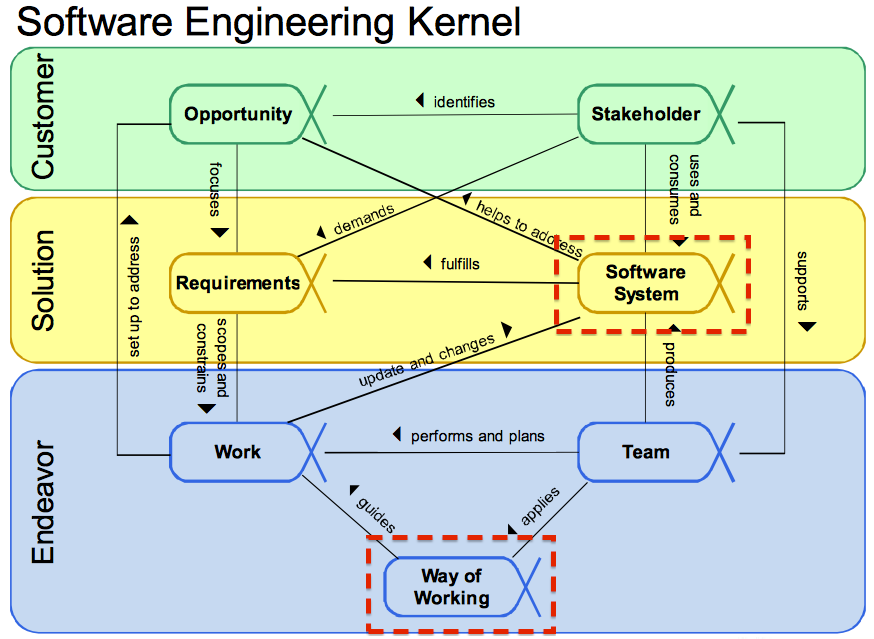
\includegraphics[width=1\textwidth]{Semat.png}
	\caption{Software Engineering Kernel}
	\end{figure}
	Di seguito viene descritto lo stato che ogni fase descritta dal \emph{Piano di Progetto} deve soddisfare, in relazione alle sezioni del \glossario{SEMAT} sopracitate.
   
   	\paragraph{Analisi}
    	\begin{itemize}
    		\item Software System:
    			\begin{enumerate}
    				\item \emph{Architecture Selected}: le piattaforme, le tecnologie e i linguaggi da usare sono stati selezionati. Vengono individuate le metriche per il software, i documenti ed i processi.
    			\end{enumerate}
    		\item Way of Working:
    			\begin{enumerate}
    				\item \emph{Principles Established}: i vincoli sono stati definiti nelle \NormeDiProgetto, i \glossario{tools} sono stati individuati ed il team comincia ad operare secondo quanto stabilito;
    				\item \emph{Foundation Established}: i \glossario{tools} per la qualità sono configurati e le buone pratiche da seguire sono definite;
    				\item \emph{In Use}: alcuni membri del team utilizzano le pratiche indicate e i tools vengono usati e migliorati. Vengono raccolti feedback sull'utilizzo degli strumenti per la qualità.
    			\end{enumerate}
    	\end{itemize}
    	
	\paragraph{Progettazione Architetturale}	
		\begin{itemize}
    		\item Software System:
    			\begin{enumerate}
    			\setcounter{enumi}{1}
    				\item \emph{Demonstrable}: le caratteristiche chiave dell'architettura software sono state individuate e gli \glossario{stakeholders} sono in accordo. Vengono individuate le unità da testare per soddisfare la richiesta del \glossario{proponente} di verificare il funzionamento di almeno il 70\% del software prodotto.
    			\end{enumerate}
    		\item Way of Working:
    			\begin{enumerate}
    			\setcounter{enumi}{3}
    				\item \emph{In Place}: tutti i membri utilizzano e comprendono l'intero ambiente di lavoro che è configurato secondo le \NormeDiProgetto. Il \glossario{repository} è configurato per accettare solo materiale in linea con le norme stabilite;
    				\item \emph{Working Well}: tutto il team lavora in modo coordinato secondo le norme applicando le pratiche individuate nelle 	norme e i \glossario{tools} supportano a pieno regime l'attività di lavoro.
    			\end{enumerate}
    			
    	\end{itemize}
    	
	\paragraph{Progettazione di Dettaglio e Codifica}	
		\begin{itemize}
    		\item Software System:
    			\begin{enumerate}
    			\setcounter{enumi}{2}
    				\item \emph{Usable}: il sistema è parzialmente usabile. Vengono praticati gli opportuni test che saranno convalidati ed il livello di anomalie sarà accettabile;
    				\item\emph{Ready}: la documentazione utente è disponibile ed è conforme alle norme. Vengono forniti i risultati dell'analisi statica e dei test eseguiti, si correggono le anomalie e gli \glossario{stakeholders} accettano il sistema.
    			\end{enumerate}
    	\end{itemize}
    	
	\paragraph{Verifica e Validazione}	
		\begin{itemize}
    		\item Software System:
    			\begin{enumerate}
    			\setcounter{enumi}{4}
    				\item \emph{Operational}: il sistema è in uso in un ambiente pienamente funzionante. Vengono ultimati gli ultimi test;
    				\item \emph{Retired}: il ritiro del software non viene considerato all'interno di questo progetto didattico.
    			\end{enumerate}
    		\item Way of Working:
    			\begin{enumerate}
    			\setcounter{enumi}{5}
    				\item \emph{Retired}: il ritiro del software non viene considerato all'interno di questo progetto didattico.
    			\end{enumerate}
    	\end{itemize}
	
		
	\subsection{Responsabilità}

	La responsabilità della verifica viene attribuita al \emph{Responsabile} di progetto e ai \emph{Verificatori}. I compiti e le modalità di attuazione sono definiti nel \emph{Piano di Progetto}.
	
	\subsection{Risorse}

	La qualifica dei processi essendo un processo, consuma delle risorse che si dividono in due categorie:
		\begin{itemize}
  			\item \textbf{Umane}: le figure coinvolte sono il \emph{Responsabile} di progetto e il \emph{Verificatore}. I processi da loro effettuati consumano ore di produttività contabilizzate e schedulate secondo il \emph{Piano di Progetto}. Le ore di produttività sono fissate dalle regole di progetto (\url{http://www.math.unipd.it/~tullio/IS-1/2013/Progetto/PD01b.html}) in un minimo di 85 e un massimo di 105 ore individuali. Il \emph{Piano di Progetto} determina la distribuzione di tali quote orarie con la relativa retribuzione. Ai fini della qualifica si potrà parlare di ore di produttività tralasciandone l'aspetto economico, in quanto non rientra nel dominio del documento succitato; 
  			
  			\item \textbf{Tecnologiche}: riguardano i \emph{mezzi} utilizzati per gli automatismi per la qualità e la loro gestione. Trattandosi esclusivamente di mezzi informatici, vengono consumate unità di calcolo considerate a costo nullo. Tale considerazione si basa sul fatto che tutti i tipi di elaborazioni informatiche sono svolte su mezzi per i quali non è richiesto né un contributo economico, né un quantitativo temporale abbastanza consistente da poter essere considerato degno di nota.
		\end{itemize}
		
	Le modalità del loro impiego sono descritte dettagliatamente nelle \emph{Norme di Progetto}.
	
%		\subsubsection{Risorse disponibili}
%		Le risorse disponibili sono tutte le \emph{risorse umane} e parte delle tecnologiche, in particolare:
%		\begin{itemize}
%			\item spazi web vari
%			\item pc portatili individuali
%		\end{itemize}
		
%		\subsubsection{Risorse necessarie}		% AWS, server per continous integration..

\iffalse		% COMMENTO
	\subsection{Strumenti}
		I \emph{tools} non disponibili ma necessari sono stati inseriti nelle \emph{Norme di Progetto}. % basta questo?
\fi

	\subsection{Tecniche}

	Le \glossario{Software Quality Managment Techinques} adottate dal gruppo sono suddivise in quattro categorie. Di seguito ne vengono date le definizioni, tuttavia non sempre si tratta di classi nettamente distinte e la loro applicazione molto spesso prevede sovrapposizioni.
	
		\subsubsection{Statiche}

		Consiste nello studiare la documentazione ed il software senza istanze di esecuzione del sorgente. Queste tecniche possono includere attività \emph{people-intensive} o di \emph{analisi} condotte da singoli individui con o senza l'assistenza di tools automatizzati.

			\paragraph{Walkthrough} \mbox{} \\
			
			Si svolge effettuando una lettura a largo spettro. È un'attività onerosa e collaborativa che richiede la cooperazione di più persone, si tratta di una tecnica non efficiente pertanto se ne sconsiglia l'attuazione. Ne è previsto l'utilizzo principalmente durante la prima parte del progetto quando non tutti i membri del gruppo hanno piena padronanza e conoscenza delle \emph{Norme di Progetto} e del \emph{Piano di Qualità}.

			\paragraph{Inspection} \mbox{} \\
			\label{anomaliefrequenti}

			Si tratta di una lettura mirata e strutturata, volta a localizzare l'errore con il minor costo possibile. Richiede una buona padronanza di tutti gli strumenti utilizzati e conoscenza di tutti i documenti di progetto. Solitamente viene effettuata da un singolo individuo. La ricerca mirata si basa sugli errori ricorrenti, uno script dovrà ricercare tali anomalie e segnalarle al \emph{Verificatore} in modo efficiente.
			Le anomalie più frequenti sono:
			\begin{itemize}
				\item utilizzo di comandi locali \LaTeX{} deprecati, ossia quei comandi che erano stati definiti alla prima creazione del \glossario{repository} ma che poi sono stati ridefiniti;
				\item utilizzo di caratteri di underscore senza prima anteporre una backslash;
				\item errori ortografici come rappresentare la \emph{È} con una \emph{e} maiuscola apostrofata;
				\item inserimento di parole comuni come placeholder, e.g. c{}i{}a{}o, b{}l{}a{}b{}l{}a, a{}s{}d \dots; % le parentesi graffe impediscono che make test-regexp trovi queste occorrenze
				\item formato delle date errato o non conforme alle \NormeDiProgetto{};
				\item formato dei nomi errato, le \NormeDiProgetto{} indicano prima il nome e poi il cognome;
				\item elenchi puntati non conformi alle norme, in particolare i punti spesso non terminano con il punto e virgola;
				

			\end{itemize}
			
			
		\subsubsection{People-intensive}

		Sono attività che coinvolgono almeno due persone impegnate a svolgere compiti anche parzialmente non automatizzabili. Solitamente l'efficienza non è massima in quanto si paga il coordinamento tra le persone. Le risorse necessarie sono checklists e i risultati dei tests e delle altre tecniche di analisi.
	
		\subsubsection{Analitiche}

		Le tecniche analitiche comprendono tutte quelle azioni volte a valutare criticamente un componente del prodotto. Tali tecniche si servono di metodi come l'analisi della complessità, degli algoritmi e del controllo di flusso. L'analisi di complessità è utile per valutare quanto un componente è articolato da progettare, implementare, testare o manutenere. Il controllo di flusso è volto al riconoscimento delle anomalie e può essere usato a supporto di altre attività. Infine, l'analisi degli algoritmi è fondamentale in quei software in cui vi è una componente algoritmica importante e vi è la necessità di assicurare output consistenti e corretti. 
				
		\subsubsection{Dinamiche}

		Le tecniche dinamiche vengono generalmente utilizzate durante lo sviluppo e la manutenzione. Si eseguono dei test ripetibili basati sull'effettiva esecuzione del codice. È quindi opportuno costruire un set di strumenti per riprodurre insiemi di \emph{input} e portare il software in uno stato iniziale, al fine di verificare velocemente che gli output siano quelli attesi. Un file di \glossario{log} permetterà, in base al contenuto, di ricostruire le sequenze di operazioni effettuate. Di seguito vengono elencati i test che si andranno ad effettuare in ordine di granularità.\\
		Il \glossario{proponente}, nel corso del primo incontro, ha indicato che dovrà essere testato almeno il  70\% del codice prodotto.
		
			\paragraph{Test di unità} \mbox{} \\

			Si tratta di testare il funzionamento delle \glossario{unità} tramite l'utilizzo di \glossario{stub}, \glossario{test driver}, e \glossario{logger}. Un'\glossario{unità} consiste nella più piccola quantità di software che è utile verificare singolarmente.
			Questi test dovrebbero procedere quanto più in parallelo, assegnando priorità alle \glossario{unità} che mostrano dei risultati utilizzabili per definire dei \glossario{prototipi}. Il corretto funzionamento di tutte le unità riduce al minimo la presenza di errori di programmazione e permette di integrare queste componenti secondo le specifiche di progetto con la garanzia che esse funzionino.
			 
			\paragraph{Test di integrazione} \mbox{} \\

			Consiste nel test di una parte di due o più \glossario{unità} e ne valuta globalmente i risultati. Le componenti non ancora sviluppate vanno simulate con dei sostituti fittizi.
			
			\paragraph{Test di sistema} \mbox{} \\

			Consiste nella validazione del sistema per accertare la copertura dei requisiti software e il suo collaudo viene supervisionato dal committente per mostrare la conformità del prodotto.
			
			\paragraph{Test di regressione} \mbox{} \\

			Consiste nell'eseguire nuovamente i test riguardanti le componenti software che hanno subito modifiche.	Tale operazione è aiutata dal tracciamento, il quale permette di individuare e ripetere facilmente i test di unità, di integrazione e di sistema che sono stati potenzialmente influenzati dalla modifica.
			
			\paragraph{Test di accettazione} \mbox{} \\

			Si tratta del collaudo del prodotto in presenza del proponente. Al superamento di tale collaudo segue il rilascio ufficiale del prodotto sviluppato.
			
	
	\subsection{Misure e Metriche}
	\label{MisureMetriche}
	
	Vengono adottate delle metriche per rendere misurabili e valutabili i processi, i documenti ed il software prodotto. La visione non vuole essere comparativa, ma serve al gruppo per monitorare l'andamento dei processi e la qualità del prodotto.
		
		\subsubsection{Metriche per i processi}
		\label{MetricheProcessi}
		Le seguenti metriche rappresentano un indicatore volto a monitorare e prevedere l'andamento delle principali variabili critiche del progetto (i tempi e i costi). Sono state scelte metriche di tipo \glossario{consuntivo} perché danno un riscontro immediato sullo stato attuale del progetto; ad ogni iterazione verranno valutati tali indici e, se necessario, verranno stabiliti opportuni provvedimenti da parte del \emph{Responsabile} di progetto.
		
			\paragraph{Schedule Variance} \mbox{} \\
			\label{ScheduleVariance}
			Indica se si è in linea, in anticipo o in ritardo rispetto alla schedulazione delle attività di progetto pianificate.
			\[
			SV = BCWP - BCWS
			\]
			Dove $BCWP$ indica valore delle attività realizzate alla data corrente e $BCWS$ rappresenta il costo pianificato per realizzare le attività di progetto alla data corrente. 
			È un indicatore di efficacia soprattutto nei confronti del Cliente. Se $SV>0$ significa che il progetto sta producendo con maggior velocità a quanto pianificato, viceversa se negativo.
			
			\paragraph{Budget Variance}\mbox{} \\
			
			Indica se alla data corrente si è speso di più o di meno rispetto a quanto previsto.
			\[
			BV = BCWS - ACWP
			\]
			Dove $BCWS$ indica il costo pianificato per realizzare le attività di  progetto alla  data corrente e $ACWP$ rappresenta costo effettivamente sostenuto alla data  corrente.
			È un indicatore che ha un valore unicamente contabile e finanziario. Se $BV>0$ significa che il progetto sta spendendo il proprio budget con minor velocità di quanto pianificato, viceversa se negativo. 

			
		\subsubsection{Metriche per i documenti}
		\label{metrichedocumenti}
		
		La \emph{leggibilità} dei documenti è indispensabile per garantirne la qualità. Si è scelto di adottare un indice per misurare la leggibilità dei testi in lingua italiana:
			
			\paragraph{Gulpease}\mbox{} \\
			\label{gulpease}
			
			L'Indice Gulpease è un indice di leggibilità di un testo tarato sulla lingua italiana. Rispetto ad altri ha il vantaggio di utilizzare la lunghezza delle parole in lettere anziché in sillabe, semplificandone il calcolo automatico. Permette di misurare la complessità dello stile di un documento.
			L'indice di Gulpease considera due variabili linguistiche: la lunghezza della parola e la lunghezza della frase rispetto al numero delle lettere.
			La formula per il suo calcolo è: \\
			$$
			89 + \frac{300 * (numero\ delle\ frasi) - 10 \cdot (numero\ delle\ lettere)}{numero\ delle\ parole}
			$$
			I risultati sono compresi tra 0 e 100, dove il valore 100 indica la leggibilità più alta e 0 la leggibilità più bassa. In generale risulta che testi con un indice:
			\begin{itemize}
				\item Inferiore a 80 sono difficili da leggere per chi ha la licenza elementare;
				\item Inferiore a 60 sono difficili da leggere per chi ha la licenza media;
				\item Inferiore a 40 sono difficili da leggere per chi ha un diploma superiore.
			\end{itemize}
			\textbf{Parametri utilizzati}:
			\begin{itemize}
				\item Range-accettazione: [40 - 100];
				\item Range-ottimale: [50 - 100].
			\end{itemize}
			
		\subsubsection{Metriche per il software}

		La prima release di \glossario{NodeJS} risale a Maggio 2009, è stata riscontrata una forte differenza tra le metriche disponibili per l'analisi statica rispetto a quelle per i linguaggi meno recenti. Inoltre, nessun membro del gruppo ha conoscenza di tale linguaggio e delle sue particolarità come l'aspetto \glossario{funzionale}. Tali differenze con i linguaggi studiati nel percorso universitario si sono tradotte nella difficoltà di individuare metriche non incentrate sulla visione ad oggetti del codice. Infine, si è osservata l'assenza di strumenti per la misurazione di metriche tradizionali come la coesione e l'instabilità dei package.
		Di seguito vengono elencate le metriche per il software prodotto.
		
			\paragraph{Complessità ciclomatica}\mbox{} \\
				
			La complessità ciclomatica è una metrica software che indica la complessità di un programma misurando il numero di cammini linearmente indipendenti attraverso il grafo di controllo di flusso. Nel grafo sopracitato i \emph{nodi} corrispondono a gruppi indivisibili di istruzioni, mentre gli \emph{archi} connettono due nodi se il secondo gruppo di istruzioni può essere eseguito immediatamente dopo il primo gruppo.
			Questo indice può essere applicato indistintamente a singole funzioni, moduli, metodi o package di un programma.
			Si vuole utilizzare tale metrica per limitare la complessità durante la fase di sviluppo.
			Durante il testing è utile per determinare il numero di casi di test necessari, infatti l'indice di complessità è un limite superiore al numero di test necessari per raggiungere il coverage completo del modulo testato. Inoltre, uno studio ha mostrato forti corrispondenze tra le metriche di complessità e il livello di coesione nei package presi in esame\footnote{Stein, C., G. Cox and L. Etzkorn, 2005. Exploring the Relationship between Cohesion and Complexity. J. Comput. Sci., 1: 137-144.}.\\
			\textbf{Parametri utilizzati}:
			\begin{itemize}
				\item Range-accettazione: [0 - 15];
				\item Range-ottimale: [0 - 10]\textsuperscript{2} .
			\end{itemize}

			
			\paragraph{Numero di metodi - NOM}\mbox{} \\
				
			Il \emph{Number of methods} è una metrica usata per calcolare la media delle occorrenze dei metodi per package. Un package non dovrebbe contenere un numero eccessivo di metodi. Valori superiori al range ottimale massimo potrebbero indicare una necessità di maggiore decomposizione del package.\\
			\textbf{Parametri utilizzati}:
			\begin{itemize}
				\item Range-accettazione: [3 - 10];
				\item Range-ottimale: [3 - 7].
			\end{itemize}

			
			\paragraph{Bugs per lines of code}\mbox{} \\
			
			% http://mayerdan.com/ruby/2012/11/11/bugs-per-line-of-code-ratio/
			Questa metrica misura il numero di bugs trovati su un certo quantitativo di linee di codice. L'aumentare del sorgente implica un incremento delle probabilità di nascondere errori, per questo è bene mantenere il codice più chiaro e semplice possibile. Con la crescita del prodotto è utile monitorare il rapporto tra i difetti trovati e il codice incrementale, tale indice dovrebbe restare costante o diminuire nel tempo.
			Il gruppo fissa questa metrica ad un massimo di 60, considerando il fatto che nessun membro ha conoscenze dello \glossario{stack} tecnologico utilizzato, l’obiettivo è di giungere alla \textit{Revisione di Accettazione} con valori compresi tra 0 e 20. Lo sforamento di tali valori determina l’intervento del \textit{Responsabile} di progetto che dovrà individuare tempestivamente la causa del problema.


			\paragraph{Variabili non utilizzate e non definite}\mbox{} \\
				
			La presenza di variabili non utilizzate viene considerata \glossario{pollution} pertanto non viene tollerata. Tali occorrenze vengono rilevate analizzando l'\glossario{Abstract syntax tree} (AST) eseguendo una cross-reference tra le variabili dichiarate e quelle inizializzate. Per sua natura, \glossario{Javascript} non blocca l'insorgenza di tali occorrenze, pertanto si rischia di dichiarare una variabile e poi utilizzarne una con nome leggermente diverso, oppure semplicemente dichiarare una variabile che in seguito non verrà mai utilizzata.\\
			\textbf{Parametri utilizzati}:
			\begin{itemize}
				\item Range-accettazione: [0 - 0];
				\item Range-ottimale: [0 - 0].
			\end{itemize}

			
			\paragraph{Numero parametri per metodo}\mbox{} \\
				
			Un numero elevato di parametri per un metodo potrebbe evidenziare un metodo troppo complesso.\\
			\textbf{Parametri utilizzati}:
			\begin{itemize}
				\item Range-accettazione: [0 - 8];
				\item Range-ottimale: [0 - 4].
			\end{itemize}
			
			
			\paragraph{Numero funzioni d'interfaccia per package}\mbox{} \\
				
			Un numero elevato di funzioni d'interfaccia in un package evidenzia un possibile errore di progettazione.\\
			\textbf{Parametri utilizzati}:
			\begin{itemize}
				\item Range-accettazione: [0 - 20];
				\item Range-ottimale: [1 - 10].
			\end{itemize}

			
			\paragraph{Halstead}\mbox{} \\
			
			La metrica di Halstead non è solamente un indice di complessità, ma identifica le proprietà misurabili del software e le relative relazioni.
			Si basa sull'osservazione che una metrica dovrebbe valutare l'implementazione di un algoritmo in linguaggi differenti ed essere indipendente dal esecuzione su una specifica piattaforma.
			In un problema vengono identificati:
			\begin{itemize}
				\item $n_1$ = il numero di operatori distinti
				\item $n_2$ = il numero di operandi distinti
				\item $N_1$ = il numero totale di operatori
				\item $N_2$ = il numero totale di operandi
			\end{itemize}
			Da cui vengono calcolati:
				\begin{itemize}
				\item $n = n_1 + n_2$: vocabolario della funzione
				\item $N = N_1 + N_2$: lunghezza della funzione
			\end{itemize}
			Data la bassa disponibilità nella rete di valori di riferimento, i range specificati sono frutto di un confronto tra il \glossario{report} sulla complessità di una libreria \glossario{open source} presa come esempio (\url{https://github.com/philbooth/complexity-report/blob/master/EXAMPLE.md}) e i valori dichiarati in \url{http://www.mccabe.com/pdf/McCabe\%20IQ\%20Metrics.pdf}. Tali valori vengono dichiarati momentanei (RR) e saranno da rivalutare sia considerando altre fonti, sia considerando i valori rilevati in parti del codice che il gruppo considera come riferimento. %TODO nelle Revisioni successive vanno controllati o aggiornati!

			
			\subparagraph{Halstead difficulty per-function}
			Il livello di difficoltà di una funzione misura la propensione all'errore ed è proporzionale al numero di operatori presenti. 
			\[
			 D = \Bigl( \frac{n1}{2} \Bigr)  * \Bigl(  \frac{N2}{n2} \Bigr)
			 \]
			\textbf{Parametri utilizzati}:
			\begin{itemize}
				\item Range-accettazione: [0 - 30];
				\item Range-ottimale: [0 - 15].
			\end{itemize}
			
			\subparagraph{Halstead volume per-function}
			Il volume descrive la dimensione dell'implementazione di un algoritmo e si basa sul numero di operazioni eseguite e sugli operandi di una funzione. Il volume di una function senza parametri composta da una sola linea è 20, mentre un indice superiore a 1000 indica che probabilmente la funzione esegue troppe operazioni.
			\[
			 V = N * \log_{2}n
			\]
			\textbf{Parametri utilizzati}:
			\begin{itemize}
				\item Range-accettazione: [20 - 1500];
				\item Range-ottimale: [20 - 1000].
			\end{itemize}

			
			\subparagraph{Halstead effort per-function}
			Lo sforzo per implementare o comprendere il significato di una funzione è proporzionale al volume a al suo livello di difficoltà.
			 \[
			 E = V * D
			\]
			\textbf{Parametri utilizzati}:
			\begin{itemize}
				\item Range-accettazione: [0 - 400];
				\item Range-ottimale: [0 - 300].
			\end{itemize}

			


\section{Gestione amministrativa della revisione}
\sectionmark{Gestione amministrativa \dots}
% APPROFONDIRE da Sommerville capitolo 24, paragrafo 24.4.2 Software compoent analisys

	\subsection{Comunicazione delle anomalie}
	\label{DefinizioneAnomalie}

	Il processo di \glossario{Software Quality Managment} è finalizzato alla ricerca dei difetti. L'identificazione delle anomalie ne permette la correzione e informa il \emph{Responsabile} di progetto sullo stato del prodotto. Distinguere e catalogare le anomalie è utile per discutere, durante revisioni e riunioni, su che correzioni attuare e con quale priorità. Di seguito vengono elencate le definizioni di anomalie (IEEE 610.12-90) adottate dal gruppo:
	\begin{itemize}
		\item \textbf{Error}: differenza riscontrata tra risultato di una computazione e valore teorico atteso (e.g. uscita dal range di accettazione degli indici di misurazione);
		\item \textbf{Fault}: un passo, un processo o un dato definito in modo erroneo (e.g. violazioni di norme tipografiche da parte di un documento). Corrisponde a quanto viene definito come \glossario{bug};
		\item \textbf{Failure}: il risultato di un \emph{fault} (e.g. incongruenza del prodotto con funzionalità indicate nell'analisi dei requisiti, incongruenza del codice con il design del prodotto);
		\item \textbf{Mistake}: azione umana che produce un risultato errato (e.g. anomalie nel repository).
	\end{itemize}
	La catalogazione delle anomalie permette l'impostazione di metriche in grado di valutarne l'andamento e in alcuni casi di predirlo, in particolare è stata scelta la metrica che conteggia il numero di \emph{bugs per lines of code}. Il \glossario{SCR} (software change request) utilizzato dal gruppo viene individuato nelle \NormeDiProgetto.


	\subsection{Controlli per la qualità di processo}
	% potrebbe evolvere in un Appendice escluisvamente dedicata alla qualità

	Le procedure di controllo per la qualità di processo sono finalizzati a migliorare la qualità del prodotto e/o diminuire i costi e tempi di sviluppo. Esistono due approcci principali:
	\begin{itemize}
		\item A maturità di processo: riflette le buone pratiche di management e tecniche di sviluppo. L'obiettivo primario è la qualità del prodotto e la prevedibilità dei processi;
		\item Agile: sviluppo iterativo senza l'overhead della documentazione e di tutti gli aspetti predeterminabili. Ha come caratteristica la responsività ai cambiamenti dei requisti cliente e uno sviluppo rapido.
	\end{itemize}

	Verrà utilizzato il primo approccio in quanto più adatto ad un team inesperto. Con una visione proattiva si cerca di avere maggior controllo e previsione sulle attività da svolgere. Questa viene anche indicata come \glossario{best practice} per gruppi poco esperti.\\
	Il processo con maggiore influenza sulla qualità del sistema non è quello di sviluppo ma è la progettazione, è qui che le capacità e le esperienze dei singoli danno un contributo decisivo.\\
	Il miglioramento dei processi è un processo ciclico composto da tre sotto processi:
	
	\begin{figure}[h]
	\centering 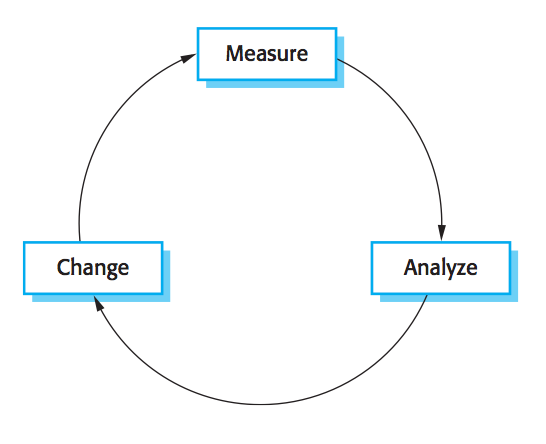
\includegraphics[width=0.8\textwidth]{ProcessImprovementCycle.png}
	\caption{Il ciclo di miglioramento dei processi}
	\end{figure}

	\begin{itemize}
		\item Misurazione del processo: misura gli attributi del progetto, punta ad allineare gli obiettivi con le misurazioni effettuate. Questo forma una \glossario{baseline} che aiuta a capire se i miglioramenti hanno avuto effetto.
		\item Analisi del processo: vengono identificate le problematiche ed i colli di bottiglia dei processi.
		\item Modifiche del processo: i cambiamenti vengono proposti in risposta alle problematiche riscontrate.
	\end{itemize}
	
	Il gruppo procederà nel seguente modo: 
	\begin{itemize}
		\item nella sezione \emph{Dettaglio delle verifiche tramite analisi} (\ref{DettaglioVerificheAnalisi}) verranno inserite le misurazioni rilevate sulle le metriche descritte in \emph{Misure e Metriche} (\ref{MisureMetriche});
		\item l'analisi viene effettuata i giorni precedenti alle consegne previste dal committente; il \emph{Riassunto delle attività di verifica} (\ref{RiassuntoAttivitaVerifica}) contiene l'analisi del processo, le relative considerazioni  comprendenti le problematiche riscontrate;
		\item le modifiche al processo vengono attuate all'inizio del processo incrementale successivo. Queste attività sono programmate nel \PianoDiProgetto.
	\end{itemize}
	
	
	
	
	

\section{Pianificazione ed esecuzione del collaudo}
Allo stato attuale non è possibile definire in dettaglio i collaudi in quanto non è stata affrontata la progettazione del prodotto, pertanto la pianificazione ed esecuzione dei collaudi saranno trattate nella prossima revisione.
	%\subsection{Specifica della campagna di validazione}
	%\subsection{Dettaglio dell'esito della campagna di validazione} %TODO da incrementare in revisioni successive!


\appendix
\addappheadtotoc
\setcounter{table}{0}
\renewcommand{\thetable}{A.\arabic{table}}

\section{Pianificazione dei test}

Si vuole adottare una strategia di verifica del software tramite test opportunamente predeterminati e che garantiscano almeno un test per ogni requisito. I test sono l'applicazione delle tecniche di verifica dinamica introdotte nelle \NormeDiProgetto{}; tali attività, oltre a richiedere l'esecuzione del programma, devono poter essere ripetibili, ossia tramite delle specifiche su come riprodurre i test vogliamo che il loro output sia deterministico. \`E importante che i test di unità vengano svolti in parallelo, dando precedenza alle unità che producono risultati utili alla comprensione del loro funzionamento integrato, l'ambiente di testing deve soddisfare tale obiettivo. \\
L'attività di test deve produrre un \glossario{log} che specifica quando e chi ha eseguito il test e con quali input; l'insorgenza di \glossario{failure} deve essere tracciata e catalogata.

	\subsection{Livelli di testing}
	Il testing del software viene suddiviso in livelli differenti e si concretizzano in un esecuzione bottom-up che avanza sequenzialmente alle attività di codifica e  di validazione. 
	I test che si andranno ad applicare sono di cinque tipi, riservando la specifica delle ultime due tipologie alla prossima revisione:

	\begin{enumerate}
		\item Test di Validazione (TV): viene verificato che il prodotto soddisfi quanto richiesto dal \glossario{proponente} individuando delle macro azioni da eseguire sul sistema che un normale utente svolge comunemente;
		\item Test di Sistema (TS): sono test relativi al comportamento dell'intero sistema ossia viene verificato che la sua architettura generale funziona complessivamente bene;
		\item Test di Integrazione (TI): vengono verificate le componenti del sistema contenute nella \SpecificaTecnica{}, ossia viene verificato che i \glossario{package} siano funzionanti e in grado di funzionare nel loro insieme; %PACKAGE
		\item Test di Unità (TU): viene testata ogni unità, ossia la più piccola parte di lavoro assegnabile ad un programmatore. In questo progetto una unità dovrebbe corrispondere ad una \code{function} o a un \code{method};  %FUNCION METODI
		\item Test di Regressione (TR): possono essere test di tutte le tipologie succitate che devono mostrare il funzionamento del prodotto a seguito di una modifica.
	\end{enumerate}

	La figura \ref{fig:V-Model} illustra come i test elencati vengono distribuiti durante in ciclo di vita del prodotto.

	\begin{figure}[H]
	\centering 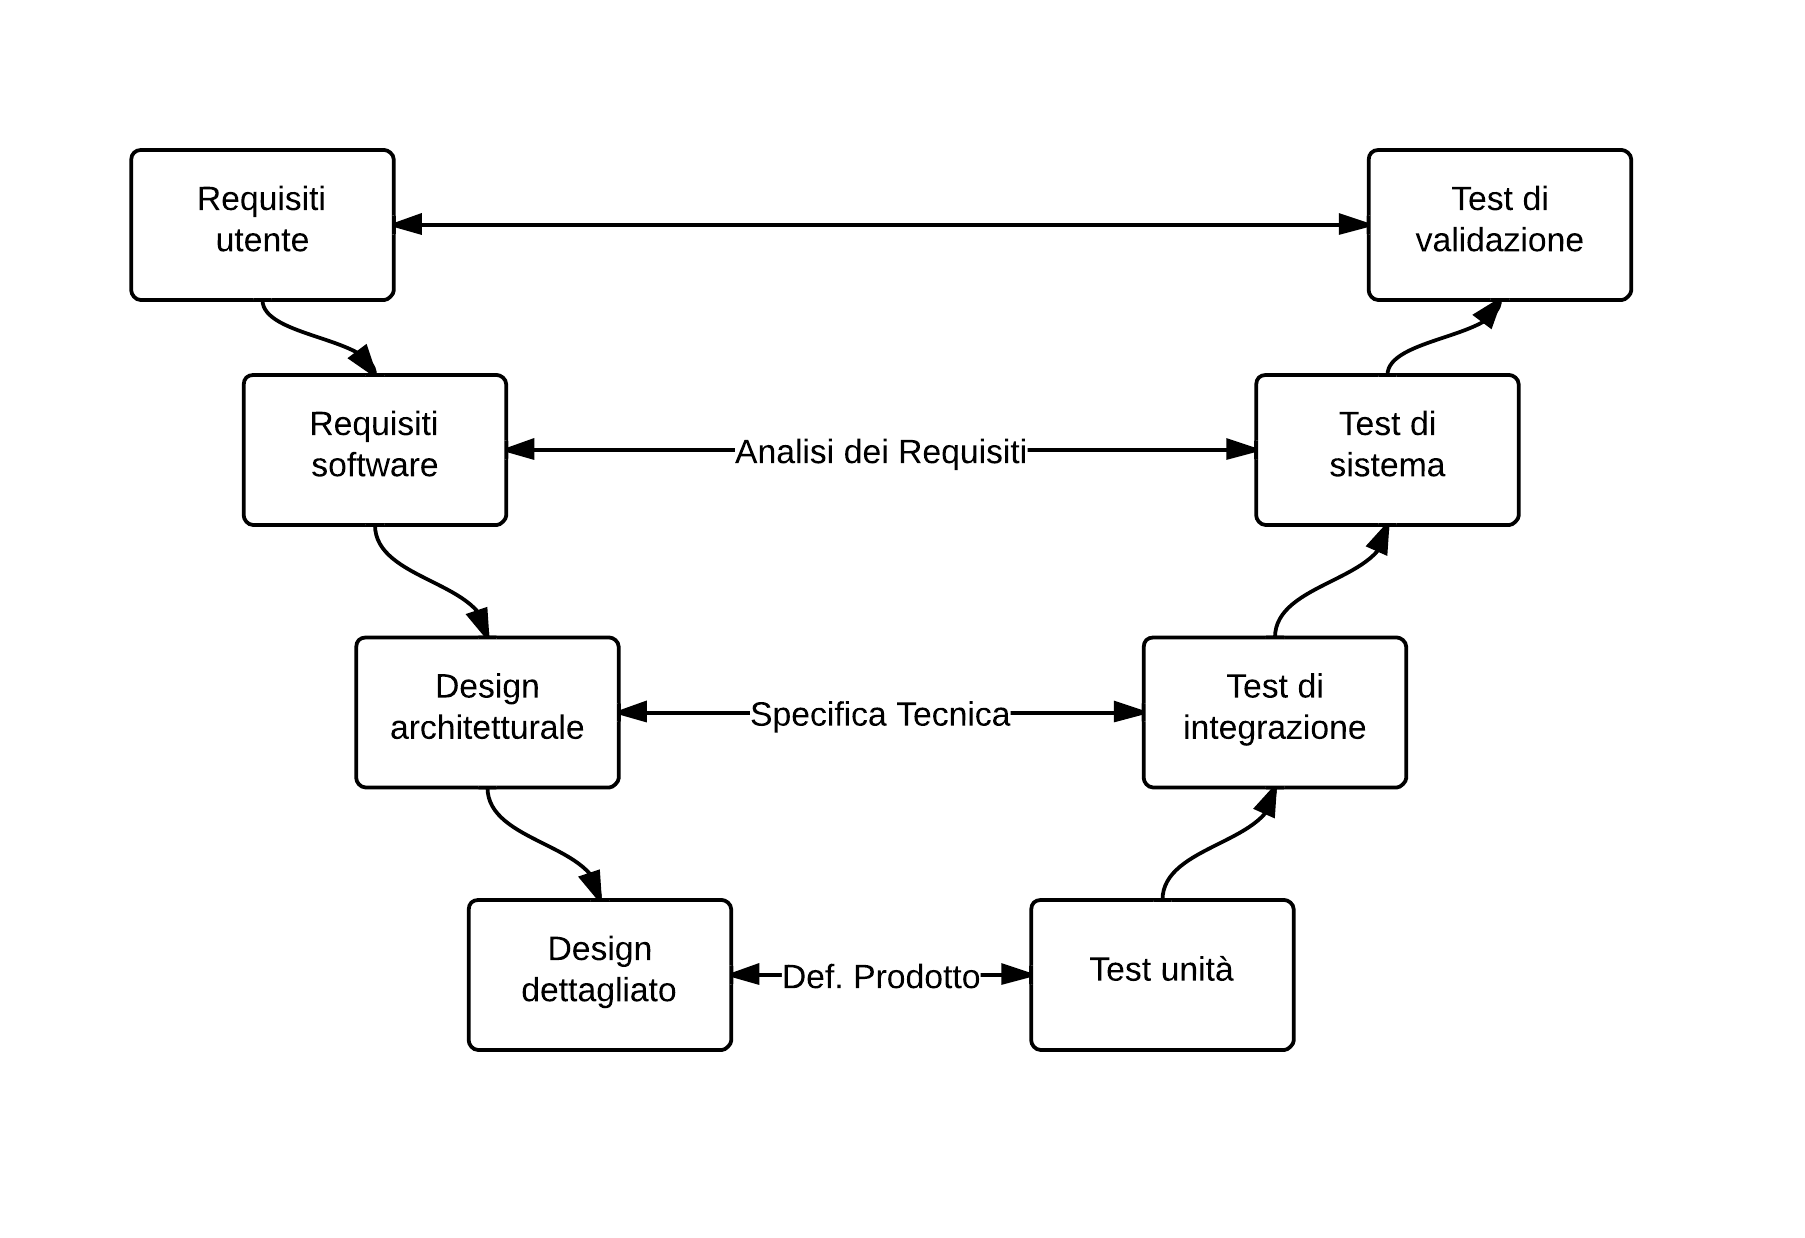
\includegraphics[width=1\textwidth]{V-Model.png}
	\caption{V-Model per il testing software}
	\label{fig:V-Model}
	\end{figure}

	\subsection{Test di sistema}
	Vengono qui descritti i test di sistema che andranno a verificare il funzionamento complessivo delle componenti.
	Nella seguente tabella, lo stato di ogni test è definito da N.E per non eseguito. I requisiti che non sono stati accettati nel \AnalisiDeiRequisiti{} sono qui marcati con un \texttt{*} ad indicare che il test associato non verrà effettuato.
	
	

	\begin{center}
	\def\arraystretch{1.5}
	\bgroup
		\begin{longtable}{| p{3cm} | p{6cm} | p{1.5cm} | p{2cm} | }
		\hline 
		 \textbf{Test Sistema} & \textbf{Descrizione} & \textbf{Stato} & \textbf{Requisito} \\ \hline
				TS-RA1O 1.1 & 
				Verificare che durante la verifica delle credenziali l'indirizzo email venga immesso tramite un campo di testo apposito. & N.E & RA1O 1.1 \newline  \\ \hline 
				TS-RA1O 1.2 & 
				Verificare che durante la verifica delle credenziali, la password venga immessa tramite un capo di testo apposito.
 & N.E & RA1O 1.2 \newline  \\ \hline 
				TS-RA1O 1.3 & 
				Verificare che il sistema verifichi le credenziali di un utente tramite un database indipendente da quello che contiene la Collection. & N.E & RA1O 1.3 \newline  \\ \hline 
				TS-RA1O 1.3.1 & 
				Verificare che, in caso di fallimento dell'autenticazione di un utente, il sistema visualizzi una pagina di errore. & N.E & RA1O 1.3.1 \newline  \\ \hline 
				TS-RA1O 1.3.2 & 
				Verificare che in caso in cui autenticazione vada a buon fine, l'utente venga reindirizzato automaticamente sulla dashboard dell'applicazione.  & N.E & RA1O 1.3.2 \newline  \\ \hline 
				TS-RA1O 2.1 & 
				Verificare che il sistema permetta il recupero password attraverso l'inserimento dell'email.
 & N.E & RA1O 2.1 \newline  \\ \hline 
				TS-RA1O 2.2 & 
				Verificare che un utente non autenticato che richiede il reset della propria password riceva un email con un link per il reset. & N.E & RA1O 2.2 \newline  \\ \hline 
				TS-RA1O 2.3 & 
				Verificare che un utente non autenticato possa resettare la propria password tramite l'inserimento di una nuova password.
 & N.E & RA1O 2.3 \newline  \\ \hline 
				TS-RA1O 4.1 & 
				Verificare che la visualizzazione di una Collection-index consista in una tabella le cui righe corrispondono ai document presenti nel database e le cui colonne siano i relativi attributi. & N.E & RA1O 4.1 \newline  \\ \hline 
				TS-RA1O 4.1.1 & 
				Verificare che ogni riga della tabella corrispondente ad un Document abbia una chiave selezionabile che rimanda alla corrispondente pagina show.
 & N.E & RA1O 4.1.1 \newline  \\ \hline 
				TS-RA1D 4.1.2 & 
				Verificare che l'admin possa eliminare un documento tramite un link rapido. & N.E & RA1D 4.1.2 \newline  \\ \hline 
				TS-RA1D 4.1.3 & 
				Verificare che l'admin possa modificare un document della collection-index.
 & N.E & RA1D 4.1.3 \newline  \\ \hline 
				TS-RA1D 4.2 & 
				Verificare che sia possibile visualizzare un sottoinsieme di Document tramite dei filtri personalizzati sugli attributi. & N.E & RA1D 4.2*  \newline  \\ \hline 
				TS-RA1F 4.3 & 
				Verificare che l'amministratore possa creare un nuovo Document nella base di dati. & N.E & RA1F 4.3*  \newline  \\ \hline 
				TS-RA1O 5.1 & 
				Verificare che l'admin possa editare ogni singolo attributo modificabile del documento della pagina show. & N.E & RA1O 5.1 \newline  \\ \hline 
				TS-RA1F 5.2 & 
				Verificare che l'utente possa eseguire un'azione personalizzata tramite l'esecuzione di un pulsante. & N.E & RA1F 5.2*  \newline  \\ \hline 
				TS-RA1O 5.3 & 
				Viene verificato che l'utente possa eliminare il Document selezionato nella show-page. & N.E & RA1O 5.3 \newline  \\ \hline 
				TS-RA1O 6.1 & 
				Viene verificato che l'admin possa creare un nuovo utente dalla pagina di amministrazione. & N.E & RA1O 6.1 \newline  \\ \hline 
				TS-RA1O 6.1.1 & 
				Viene verificato che l'admin disponga di una pagina di creazione di un nuovo utente. & N.E & RA1O 6.1.1 \newline  \\ \hline 
				TS-RA1O 6.1.1.1 & 
				Verificare che l'admin possa inserire l'indirizzo email del nuovo utente in un apposito campo di testo presente all'interno della pagina di creazione di un nuovo utente. & N.E & RA1O 6.1.1.1 \newline  \\ \hline 
				TS-RA1O 6.1.1.2 & 
				Viene verificato che l'admin possa inserire la password del nuovo utente in un apposito campo di testo presente all'interno della pagina di creazione di un nuovo utente. & N.E & RA1O 6.1.1.2 \newline  \\ \hline 
				TS-RA1O 6.1.1.3 & 
				Verificare che l'admin possa inserire il ``livello utente'' del nuovo utente tramite una combo-box presente all'interno della pagina di creazione di un nuovo utente. & N.E & RA1O 6.1.1.3 \newline  \\ \hline 
				TS-RA1O 6.1.2 & 
				Viene verificato che l'applicazione prelevi tutti i dati inseriti dall'admin nella pagina di creazione di un nuovo utente e li invii al database delle credenziali, il quale provvederà all'inserimento del nuovo record. & N.E & RA1O 6.1.2 \newline  \\ \hline 
				TS-RA1O 6.1.3 & 
				Verificare che venga visualizzato un messaggio d'errore nel caso in cui l'admin non abbia compilato correttamente i campi presenti all'interno della pagina di creazione di un nuovo utente. & N.E & RA1O 6.1.3 \newline  \\ \hline 
				TS-RA1O 6.2 & 
				Viene verificato che l'admin abbia la possibilità di selezionare un utente dalla index-page e visualizzare la sua relativa show-page. & N.E & RA1O 6.2 \newline  \\ \hline 
				TS-RA1O 6.2.1 & 
				Verificare che l'admin possa elevare l'utente normale selezionato al livello ``admin'' dalla show-page relativa. & N.E & RA1O 6.2.1 \newline  \\ \hline 
				TS-RA1O 6.2.2 & 
				Verificare che l'admin possa declassare l'admin selezionato a livello di utente normale dalla show-page relativa. & N.E & RA1O 6.2.2 \newline  \\ \hline 
				TS-RA1O 6.2.3 & 
				Viene verificato che l'admin possa modificare l'attributo email dell'utente selezionato dalla relativa show-page. & N.E & RA1O 6.2.3 \newline  \\ \hline 
				TS-RA1O 6.2.4 & 
				Verificare che l'admin possa modificare l'attributo password dell'utente selezionato dalla relativa show-page. & N.E & RA1O 6.2.4 \newline  \\ \hline 
				TS-RA1O 6.2.5 & 
				Viene verificato che l'admin possa eliminare l'utente visualizzato nella \glossario{show-page}. & N.E & RA1O 6.2.5 \newline  \\ \hline 
				TS-RF1O 7 & 
				Verificare che il linguaggio DSL all'interno di MaaP Framework sia stato implementato e sia funzionante. & N.E & RF1O 7 \newline  \\ \hline 
				TS-RF1O 8.1  & 
				Verificare che Maap Framework generi automaticamente lo scheletro dell’applicazione creata dallo sviluppatore. & N.E & RF1O 8.1  \newline  \\ \hline 
				TS-RF1O 8.1.1 & 
				Verificare che Maap Framework importi automaticamente in un'apposita directory del progetto tutte le librerie necessarie al corretto funzionamento del sistema. Librerie necessarie: \begin{itemize} \item Express v-3.4.8 \item MongoDB v-1.3.23 \item Mongoose v-3.8.4 \end{itemize} & N.E & RF1O 8.1.1 \newline  \\ \hline 
				TS-RF1O 8.1.2 & 
				Verificare che Maap Framework crei automaticamente in un’apposita directory il file di configurazione di default dell’applicazione generata. & N.E & RF1O 8.1.2 \newline  \\ \hline 
				TS-RF1O 8.1.3 & 
				Viene verificato che Maap Framework crei automaticamente il sistema di autenticazione per l’applicazione generata. & N.E & RF1O 8.1.3 \newline  \\ \hline 
				TS-RF1O 8.1.4 & 
				Verificare che Maap Framework crei automaticamente le directory di descrizione delle pagine web. & N.E & RF1O 8.1.4 \newline  \\ \hline 
				TS-RF1O 8.2 & 
				Verificare che Maap Framework crei automaticamente un account admin di default. & N.E & RF1O 8.2 \newline  \\ \hline 
				TS-RF1F 8.3 & 
				Verificare che il framework MaaP permetta allo sviluppatore di definire un namespace per l’applicazione generata. & N.E & RF1F 8.3*  \newline  \\ \hline 
				TS-RF1O 9.1 & 
				Verificare che il DSL permetta allo sviluppatore di creare una pagina Collection-index. & N.E & RF1O 9.1 \newline  \\ \hline 
				TS-RF1O 9.1.1 & 
				Verificare che il DSL deve permetta allo sviluppatore di poter definire una serie di attributi da visualizzare all’interno della pagina Collection-index. & N.E & RF1O 9.1.1 \newline  \\ \hline 
				TS-RF1O 9.1.2 & 
				Viene verificato che il DSL permetta allo sviluppatore di poter definire un ordinamento di default (ordine alfanumerico) di visualizzazione dei document all'interno della pagina Collection-index. & N.E & RF1O 9.1.2 \newline  \\ \hline 
				TS-RF1O 9.1.3 & 
				Verificare che il DSL permetta allo sviluppatore di poter definire un eventuale limite di elementi da visualizzare all’interno della pagina Collection-index. & N.E & RF1O 9.1.3 \newline  \\ \hline 
				TS-RF1O 9.1.4 & 
				Viene verificato che il DSL permetta allo sviluppatore di poter definire quali attributi sono ordinabili all’interno della pagina Collection-index. & N.E & RF1O 9.1.4 \newline  \\ \hline 
				TS-RF1O 9.1.5 & 
				Verificare che il DSL permetta allo sviluppatore di definire la funzione populate per far si che una chiave riferisca ad un documento esterno. & N.E & RF1O 9.1.5 \newline  \\ \hline 
				TS-RF1O 9.1.6 & 
				Verificare che il DSL permetta allo sviluppatore di definire delle query per creare la pagina Collection-index in base al risultato della loro estrazione. & N.E & RF1O 9.1.6 \newline  \\ \hline 
				TS-RF1O 9.1.7 & 
				Viene verificato che il DSL permetta allo sviluppatore di definire delle trasformazioni sugli attributi da visualizzare. & N.E & RF1O 9.1.7 \newline  \\ \hline 
				TS-RF1O 9.2 & 
				Viene verificato che il DSL permetta allo sviluppatore di creare una pagina Collection-show. & N.E & RF1O 9.2 \newline  \\ \hline 
				TS-RF1O 9.2.1 & 
				Verificare che il DSL permetta allo sviluppatore di definire una serie di attributi visualizzabili all’interno della pagina Collection-show. & N.E & RF1O 9.2.1 \newline  \\ \hline 
				TS-RF1O 9.2.2 & 
				Verificare che il DSL permetta allo sviluppatore la definizione degli attributi del Document come attributi innestati o array di Document tramite la funzione populate. & N.E & RF1O 9.2.2 \newline  \\ \hline 
				TS-RF1O 9.2.3 & 
				Verificare che lo sviluppatore abbia la possibilità di personalizzare la show page definendone l’ordinamento degli attributi. & N.E & RF1O 9.2.3 \newline  \\ \hline 
				TS-RF1O 9.2.4 & 
				Viene verificato che lo sviluppatore possa definire trasformazioni agli attributi per poi visualizzarli nella show-page. & N.E & RF1O 9.2.4 \newline  \\ \hline 
				TS-RF1F 9.2.5 & 
				Verificare che lo sviluppatore possa personalizzare la show-page definendo delle operazioni personalizzate che l’utente potrà utilizzare tramite appositi pulsanti. & N.E & RF1F 9.2.5*  \newline  \\ \hline 
				TS-RF1O 9.3 & 
				Viene verificato che il framework MaaP permetta allo sviluppatore di cambiare il nome della Collection da visualizzare nel menu di navigazione. & N.E & RF1O 9.3 \newline  \\ \hline 
				TS-RF1O 9.4 & 
				Verificare che il framework MaaP permetta allo sviluppatore di modificare l’ordine di visualizzazione della Collection nel menu di navigazione. & N.E & RF1O 9.4 \newline  \\ \hline 
				TS-RS1F 10.1 & 
				Verificare che il sistema MaaS permetta allo sviluppatore di scrivere una Collection tramite editor di testo presente nella pagina web. & N.E & RS1F 10.1*  \newline  \\ \hline 
				TS-RS1F 10.2 & 
				Verificare che il sistema MaaS permetta all'utente di poter scrivere una Collection caricando un file prodotto dal framework MaaP. & N.E & RS1F 10.2*  \newline  \\ \hline 
				TS-RS1F 10.3 & 
				Verificare che il sistema MaaS permetta ad un utente non registrato di registrarsi al suo servizio. & N.E & RS1F 10.3*  \newline  \\ \hline 
				TS-RS1F 10.4 & 
				Verificare che il sistema MaaS assegni automaticamente un \glossario{namespace} sul sistema al nuovo utente registrato. & N.E & RS1F 10.4*  \newline  \\ \hline 
				TS-RS1F 10.5 & 
				Verificare che il servizio MaaS visualizzi un messaggio d’errore nel caso in cui la registrazione fallisca a causa di credenziali già esistenti. & N.E & RS1F 10.5*  \newline  \\ \hline 
				TS-RS1F 10.6 & 
				Verificare che il servizio MaaS metta a disposizione di un utente non autenticato la possibilità di effettuare il login al sistema. & N.E & RS1F 10.6*  \newline  \\ \hline 
				TS-RS1F 10.7 & 
				Verificare che il servizio MaaS visualizzi un messaggio d’errore nel caso in cui l’utente non autenticato abbia inserito credenziali errate nel sistema di login. & N.E & RS1F 10.7*  \newline  \\ \hline 
				TS-RS1F 10.8 & 
				Verificare che il sistema MaaS permetta ad un utente non autenticato di modificare il proprio profilo. & N.E & RS1F 10.8*  \newline  \\ \hline 
				TS-RS1F 10.9 & 
				Verificare che il sistema MaaS permetta ad un utente non autenticato di eliminare il proprio account dal sistema. & N.E & RS1F 10.9*  \newline  \\ \hline 
				TS-RS1F 10.9.1 & 
				Verificare che il sistema MaaS provveda all'eliminazione dei file di configurazione associati all'utente rimosso dal sistema. & N.E & RS1F 10.9.1*  \newline  \\ \hline 
				TS-RS1F 10.10 & 
				Verificare che il sistema MaaS permetta allo sviluppatore di eliminare una Collection esistente. & N.E & RS1F 10.10*  \newline  \\ \hline 
				TS-RA1D 13.1 & 
				Verificare che l’utente possa modificare la password di accesso all'applicazione. & N.E & RA1D 13.1 \newline  \\ \hline 
				TS-RF1O 14.1 & 
				Verificare che il framework MaaP renda possibile la configurazione dei database delle credenziali. & N.E & RF1O 14.1 \newline  \\ \hline 
				TS-RF1O 14.2 & 
				Verificare che il framework MaaP renda possibile la configurazione dei database delle Collection. & N.E & RF1O 14.2 \newline  \\ \hline 
				TS-RF1F 14.3 & 
				Verificare che il framework MaaP renda possibile la selezione di un name-space per un database se la funzione di \glossario{namespace} è abilitata. & N.E & RF1F 14.3*  \newline  \\ \hline 
				TS-RA1F 15.1 & 
				Verificare che l’applicazione MaaP metta a disposizione dell’admin la visualizzazione degli indici in base alle query più richieste dall’applicazione. & N.E & RA1F 15.1*  \newline  \\ \hline 
				TS-RA1F 15.2 & 
				Verificare che l’applicazione MaaP permetta all’admin di aggiungere gli indici in base ai suggerimenti forniti. & N.E & RA1F 15.2*  \newline  \\ \hline 
				TS-RA1F 15.3 & 
				Verificare che l’applicazione MaaP permetta all’admin di rimuovere gli indici in base ai suggerimenti forniti. & N.E & RA1F 15.3*  \newline  \\ \hline 
				TS-RS1F 17 & 
				Verificare che Il sistema MaaS si accerti che documenti creati rispettano i vincoli del database. & N.E & RS1F 17*  \newline  \\ \hline 
				TS-RA1O 18 & 
				Verificare che il sistema metta a disposizione un validatore del codice DSL e visualizzi gli eventuali errori logici o di sintassi in un'apposita pagina. & N.E & RA1O 18 \newline  \\ \hline 
				TS-RS1F 19 & 
				Verificare che il sistema MaaS salvi le pagine definite dagli utenti nel database e non su disco. & N.E & RS1F 19*  \newline  \\ \hline 
		\caption{Tracciamento Test di Sistema - Requisiti}
		\end{longtable}
	 \egroup
\end{center}
	
	\subsection{Test di integrazione}
	I test di integrazione vanno a controllare il corretto funzionamento delle componenti descritti dalla progettazione ad alto livello. Si è scelto di utilizzare un approccio \glossario{top-down} ad eccezione del test TI 9 che viene eseguito con la metodologia \glossario{bottom-up}. Di seguito viene riportato un diagramma informale per chiarire l'albero dei test di integrazione.

	\begin{figure}[H]
	\centering 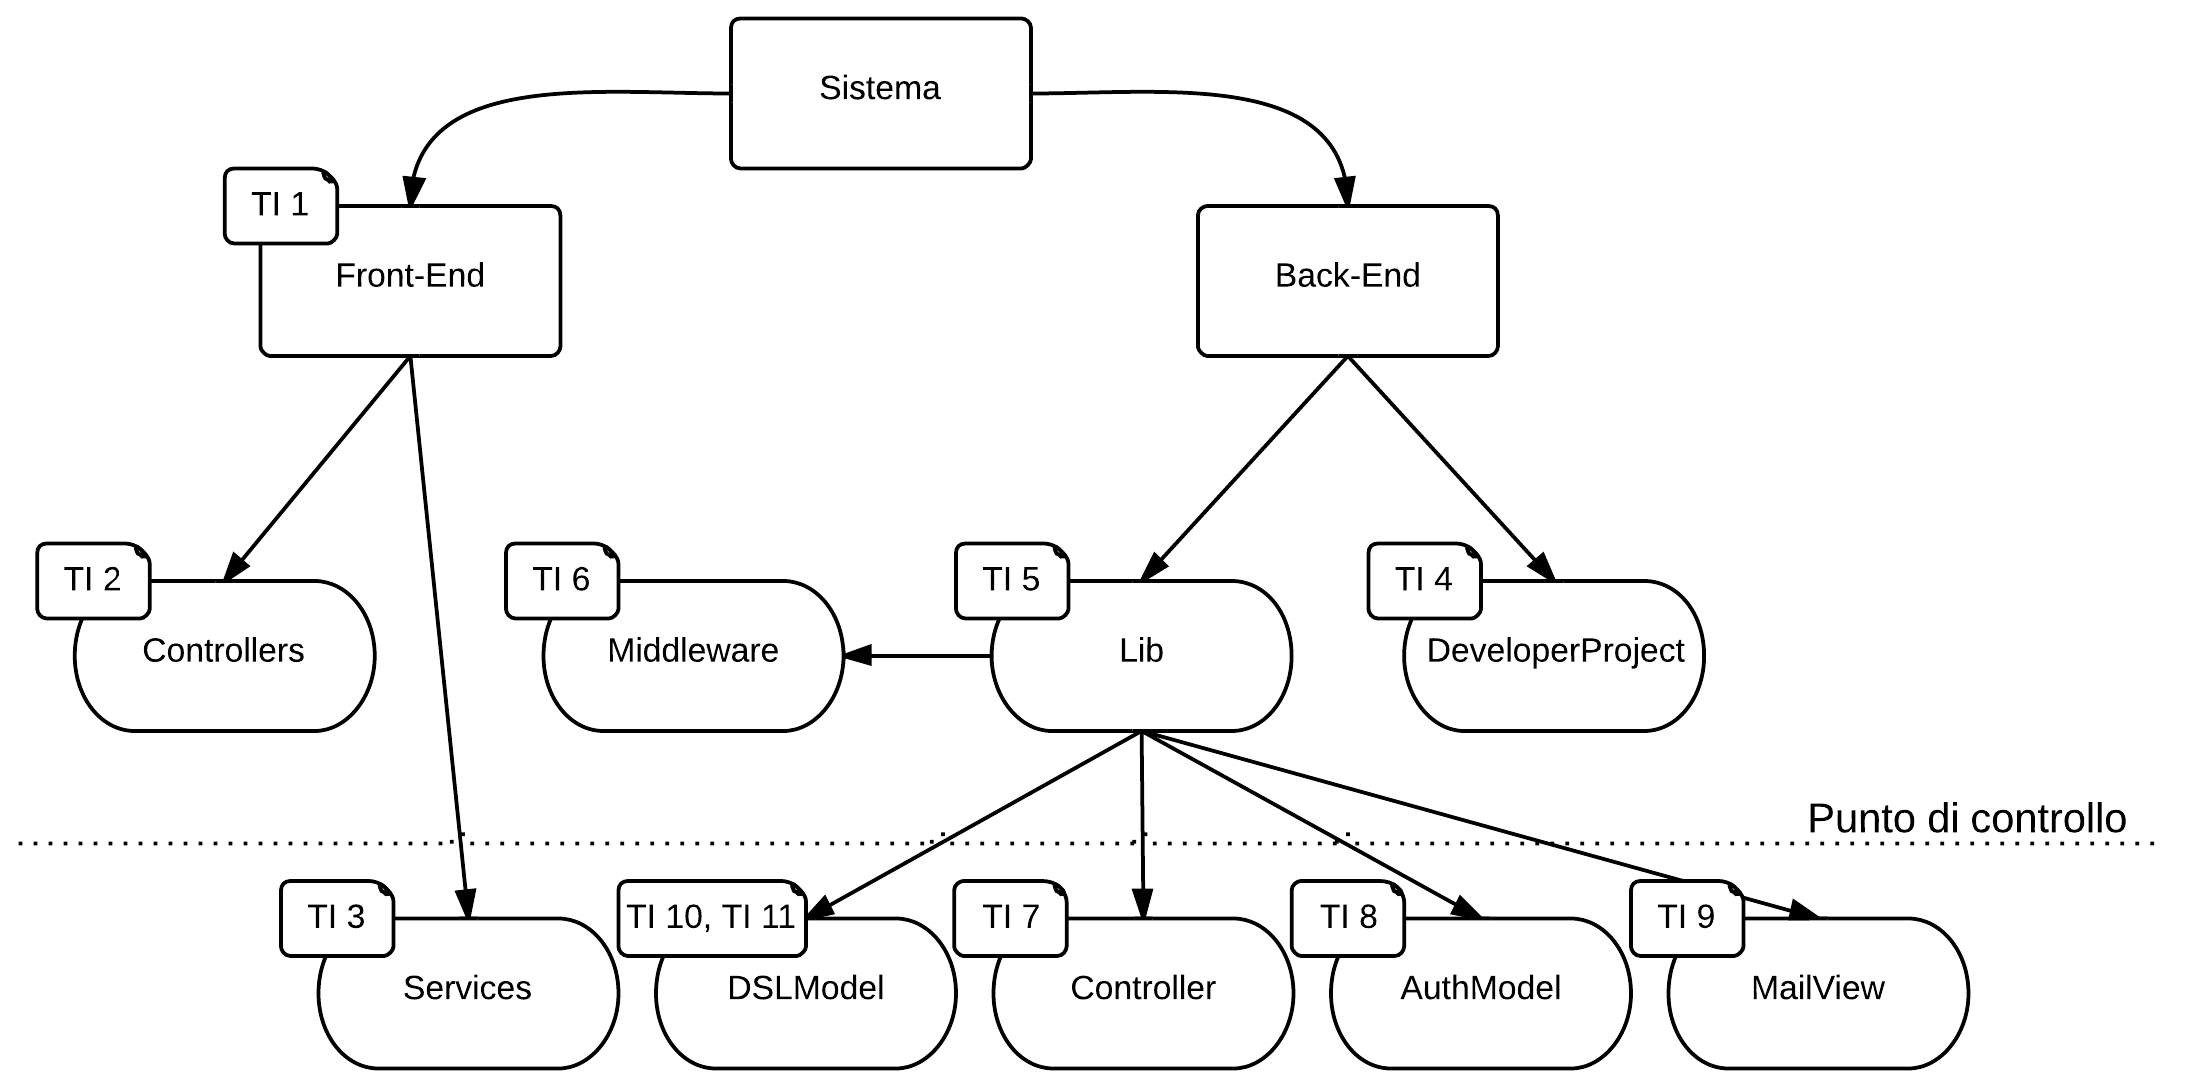
\includegraphics[width=1\textwidth]{sequenza-di-integrazione.png}
	\caption{Sequenza d'integrazione delle componenti}
	\label{fig:sequenza-di-integrazione}
	\end{figure}

	Con la tecnica \glossario{top-down} le componenti di più alto livello sono testate non appena sono implementate. Le componenti del sottosistema che non sono ancora state sviluppate, vengono simulate dagli \glossario{stub}. Man mano che si procede con la codifica delle componenti di più basso livello, queste vengono integrate e viene eseguito il relativo test. Grazie all'integrazione incrementale delle componenti del sistema, è più semplice determinare quale componente crea problemi e le funzioni di più alto livello sono testate prima.

	La componente Front-end::Model non ha associato test d'integrazione poiché le classi di questo \glossario{package} si prevede che non verranno codificate in quanto verrà sfruttato lo stile di \glossario{duck-typing} della gestione dei tipi di \glossario{JavaScript}.

	\begin{figure}[H]
	\centering 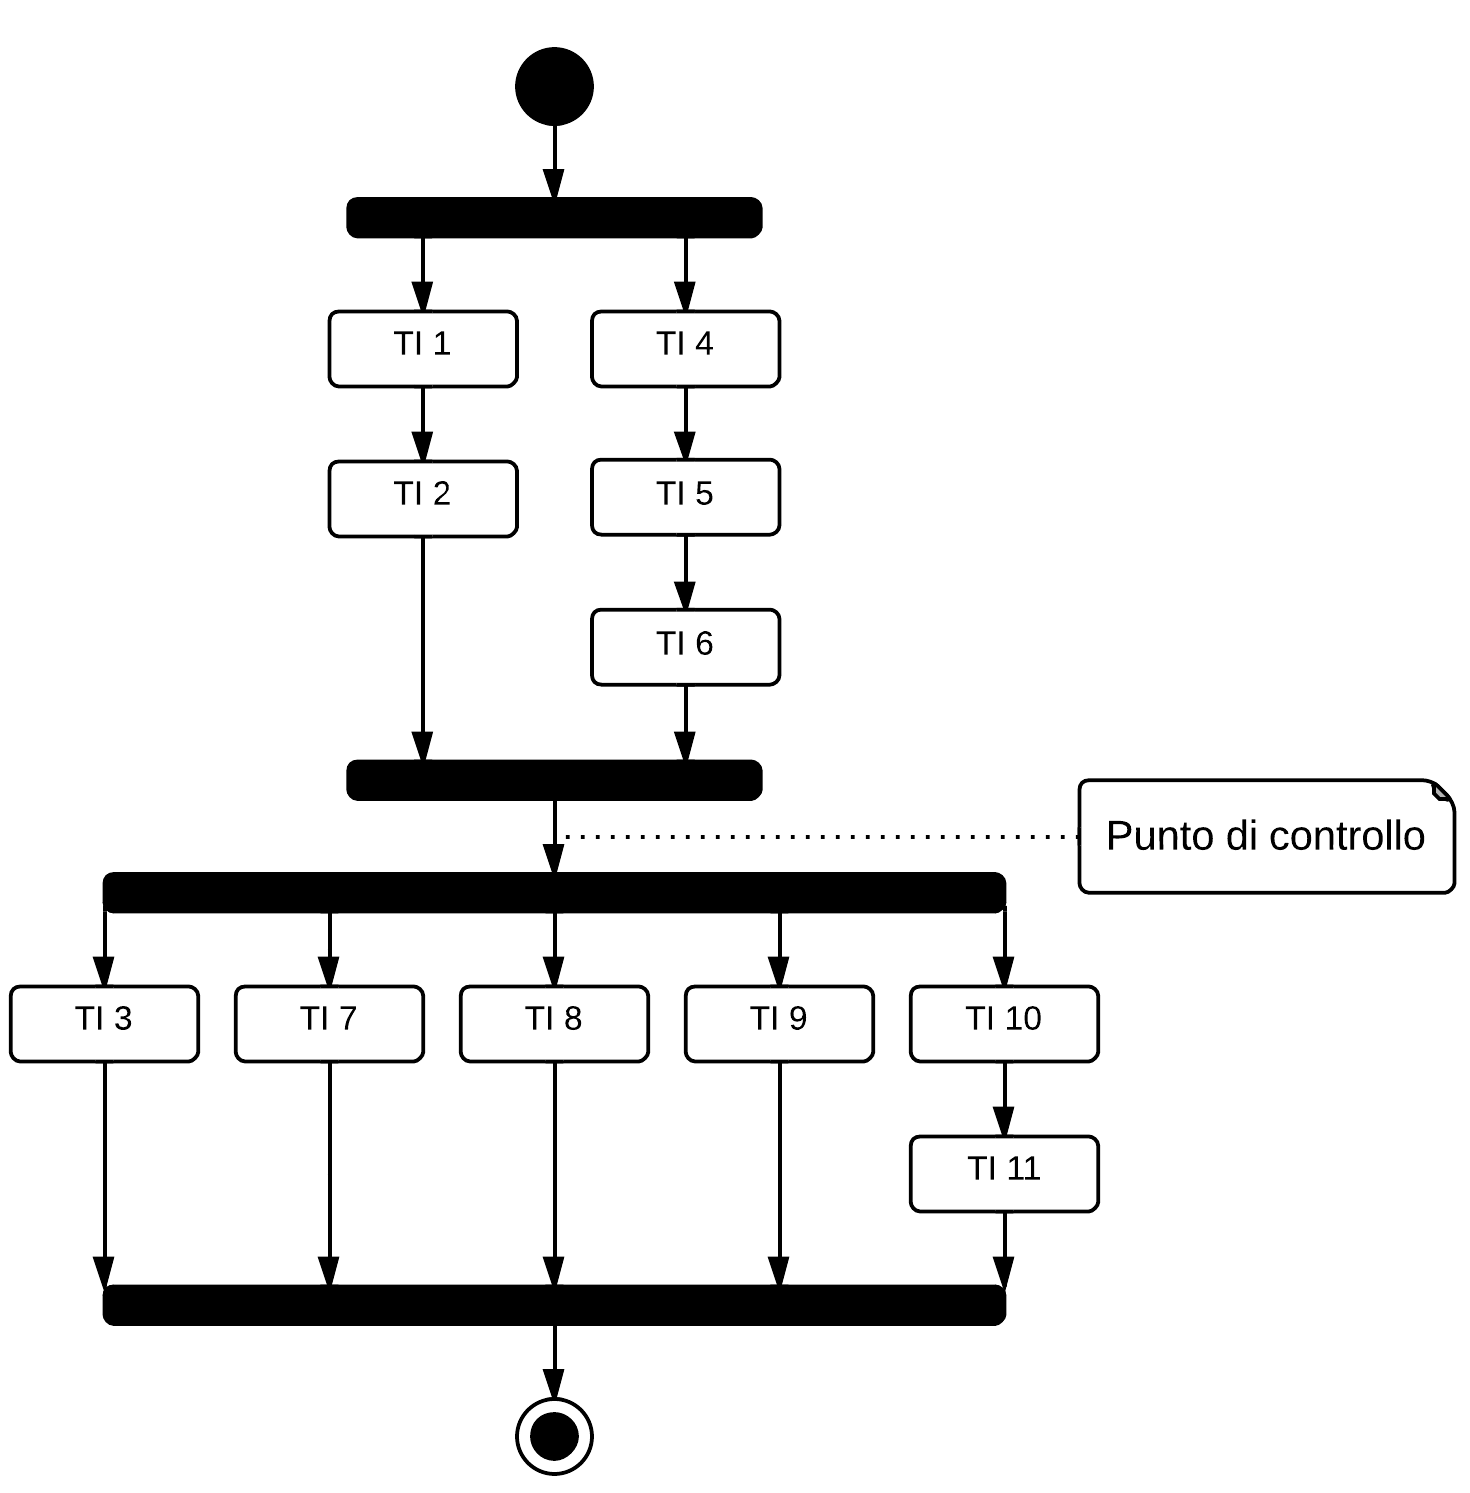
\includegraphics[width=0.59\textwidth]{sequenza-dei-test.png}
	\caption{Diagramma di attività dei test}
	\label{fig:sequenza-dei-test}
	\end{figure}
	
	%TODO tabella: componente / test
	\bgroup
	\begin{longtable}[H]{|P{1cm}|P{5cm}|P{4.5cm}|P{2cm}|}
		\hline \textbf{Test} & \textbf{Descrizione} & \textbf{Componenti aggiunte} & \textbf{Stato} \\
		
		\hline TI 1 & Si verifica che l'applicazione Web carichi correttamente le librerie JavaScript utilizzate. & Front-end & N.E. \\
		\hline TI 2 & Si verifica che i controller si integrino correttamente nell'applicazione Web. & Front-end::Controllers & N.E. \\
		\hline TI 3 & Si verifica che i services permettono di interagire correttamente con il back-end. & Front-end::Services & N.E. \\
		\hline TI 4 & Si verifica che il DeveloperProject avvii correttamente il server, fornendo in particolare i file statici del front-end. & Back-end::DeveloperProject & N.E. \\
		\hline TI 5 & Si verifica che la libreria si integri correttamente con il \glossario{Node Package Manager} (npm) E che il suo script di installazione produca un DeveloperProject funzionante. & Back-end::Lib & N.E. \\
		\hline TI 6 & Si verifica che i controller si integrino correttamente tra loro e nella gestione delle richieste che arrivano al server. & Back-end::Lib::Controller & N.E. \\
		\hline TI 7 & Si verifica che il Middleware si integri correttamente nella gestione delle richieste che arrivano al server. & Back-end::Lib::Controller::Middleware & N.E. \\
		\hline TI 8 & Si verifica che il Service si integri correttamente nella gestione delle richieste che arrivano al server. & Back-end::Lib::Controller::Service & N.E. \\
		\hline TI 9 & Si verifica che il Model si integri correttamente della gestione dell'inserimento, della modifica, della creazione e dell'eliminazione consistente dei dati. & Back-end::Lib::Model & N.E. \\
		\hline TI 10 & Si verifica che la View si integri correttamente con il Middleware per fornire i template come la gestione dell'invio delle mail. & Back-end::Lib::View & N.E. \\
		\hline TI 11 & Si verifica che Utils si integri correttamente con il funzionamento dell'applicazione. & Back-end::Lib::Utils & N.E. \\
		\hline TI 12 & Si verifica che le classi che compongono il DSLModel interagiscano correttamente tra loro. & Back-end::Lib::DSLModel & N.E. \\
		\hline TI 13 & Si verifica che il DSLModel si integri correttamente con il funzionamento dell'applicazione. & Back-end::Lib::DSLModel & N.E. \\
		\hline

	\caption{Descrizione test d'Integrazione}
	\end{longtable}
	\egroup

	\subsection{Test di validazione}
	In questa sezione vengono elencati i test di validazione per verificare che il prodotto sia conforme alle attese. I test si svolgono seguendo e verificano tutti passi di cui si compongono. I requisiti che non sono stati accettati nel \AnalisiDeiRequisiti{} sono qui marcati con un \texttt{*} ad indicare che il test associato non verrà effettuato.
	
	
  \begin{center}
  \def\arraystretch{1.5}
  \bgroup
    \begin{longtable}{| p{3cm} | p{6cm} | p{1.5cm} | p{2cm} | }
    \hline 
     \textbf{Test di Validazione} & \textbf{Descrizione} & \textbf{Stato} & \textbf{Requisito} \\ \hline
        TV-RA1O 1 & 
        L'utente non autenticato intende accedere all'applicazione, per farlo deve inserire le proprie credenziali composte da una email ed una password.
All'utente è richiesto di:
\begin{itemize}
\item Raggiungere la pagina di autenticazione;
\item Inserire la mail nel campo apposito;
\item Inserire la password;
\item Procedere con l'autenticazione.
\end{itemize}
 & N.E &       
            RA1O 1 \newline  \\ \hline 
        TV-RA1O 2 & 
        L'utente intende recuperare la password d'accesso all'applicazione.
All'utente è richiesto di:
\begin{itemize}
\item Essere autenticato;
\item Raggiungere la pagina per il reset della password;
\item Richiedere il reset;
\item Raggiungere la casella email collegata all'account del sistema;
\item Seguire il link contento nella mail:
\item Compilare il form richiedente la nuova password;
\item Eseguire il Logout e autenticarsi con la nuova password.
\end{itemize} & N.E &       
            RA1O 2 \newline  \\ \hline 
        TV-RA1D 3 & 
        L'utente autenticato può visualizzare la pagina di Dashboard nella quale potrà aver accesso ad esempio alla lista delle collection presenti e ad altre funzionalità disponibili.
All'utente è richiesto di:
\begin{itemize}
\item Accertarsi di essere autenticato;
\item Accedere alla pagina Dashboard tramite il menu di navigazione;
\end{itemize} & N.E &       
            RA1D 3 \newline  \\ \hline 
        TV-RA1O 4 & 
        L'utente autenticato, selezionata una \glossario{Collection}, ne visualizza in forma tabellare tutti i documenti che contiene. \newline Di questa collection può filtrarne i risultati visualizzabili, può eseguire tramite bottoni predisposti nella pagina azioni personalizzati e per ogni \glossario{Document}, selezionarlo e visualizzarne la show-page corrispondente. \newline L'Admin ha i permessi per modificare un documento o eliminare un \glossario{Document}. \newline
All'utente è richiesto di:
\begin{itemize}
\item Essere autenticato;
\item Aprire la show-page relativa ad un Document;
\item Usare i filtri per filtrare la Collection
\item Eseguire un azione personalizzata, laddove presente;
\item Se admin, modificare un Document;
\item Se admin, eliminare un Document;
\end{itemize} & N.E &       
            RA1O 4 \newline  \\ \hline 
        TV-RA1O 5 & 
        L'utente visualizza la pagina show-page corrispondente ad un \glossario{Document} selezionato visualizzandone gli attributi in forma tabellare. \newline In questa pagina può aprire la show-page o l'index-page dell'array di \glossario{Document} degli attributi innestati se presenti, eseguire un'operazione personalizzata se disponibile. \newline L'Admin può eliminare il \glossario{Document} a cui la show-page corrisponde o modificarlo. 
All'utente è richiesto di:
\begin{item}
\item Essere autenticato;
\item Aprire la show-page degli attributi innestati;
\item Aprire l'index-page dell'arra di Document;
\item Eseguire, se presente, un operazione personalizzata;
\item Se admin, modificare il Document;
\item Se admin, eliminare il Document.
\end{item} & N.E &       
            RA1O 5 \newline  \\ \hline 
        TV-RA1O 6 & 
        L'Admin entra nella sua pagina di amministrazione nella quale visualizza una \glossario{Collection-Index} di tutti gli utenti registrati al sistema.
All'utente è richiesto di:
\begin{itemize}
\item Essere autenticato come admin;
\item Accedere alla pagina di creazione nuovi utenti;
\item Creare un nuovo utente;
\item Accedere alla pagina degli utenti registrati al sistema;
\item Visualizzare la pagina Collection-Show di un utente;
\end{itemize}
 & N.E &       
            RA1O 6 \newline  \\ \hline 
        TV-RF1O 8 & 
        Lo sviluppatore deve poter creare un nuovo progetto tramite linea di comando.
\newline
Allo sviluppatore è richiesto di:
\begin{itemize}
\item Richiamare il comando di creazione di un nuovo progetto;
\item Passare come parametro il nome della directory che conterrà il progetto;
\item Verificare che siano state importate le librerie necessarie al corretto funzionamento del sistema;
\item Verificare che sia stato creato il file di configurazione di default dell’applicazione generata;
\item Verificare che sia stato creato il sistema di autenticazione per l’applicazione generata;
\item Verificare che siano state create le directory di descrizione delle pagine web;
\item Verificare che sia stato creato un account admin di default.
\end{itemize} & N.E &       
            RF1O 8 \newline  \\ \hline 
        TV-RF1O 9 & 
        Lo sviluppatore deve poter configurare le Collection tramite il DSL di Maap Framework.
All'utente è richiesto di:
\begin{itemize}
\item creare una Collection-index tramite DSL;
\item creare una Collection-show tramite DSL;
\item modificare il nome della Collection;
\item modificare l'ordine di visualizzazione della Collection.
\end{itemize} & N.E &       
            RF1O 9 \newline  \\ \hline 
        TV-RS1F 10 & 
        L'utente autenticato verifica che il \glossario{framework} MaaP sia messo a disposizione dal sistema \glossario{MaaS} come servizio Web.
\newline
All'utente è richiesto di:
\begin{itemize}
\item Accedere alla pagina di modifica del proprio profilo;
\item Modificare i dati associati al proprio profilo;
\item Verificare che i dati siano stati aggiornati;
\item Gestire i file di configurazione;
\item Eliminare il proprio account;
\item Verificare l'inaccessibilità al servizio tramite l'autenticazione con le credenziali associate all'account eliminato.
\end{itemize} & N.E &       
            RS1F 10 \newline  \\ \hline 
        TV-RA1D 11 & 
        L'utente non autenticato deve potersi registrare all'applicazione MaaP.
\newline
All'utente è richiesto di:
\begin{itemize}
\item Inserire la mail nell'apposito campo di testo;
\item Inserire la password nell'apposito campo di testo;
\item Verificare che l'account sia stato registrato tramite l'autenticazione all'applicazione.
\end{itemize} & N.E &       
            RA1D 11 \newline  \\ \hline 
        TV-RA1D 12 & 
        L'utente autenticato deve poter eseguire il logout dall'applicazione.
\newline
All'utente è richiesto di:
\begin{itemize}
\item Selezionare l'apposita opzione di logout;
\item Verificare di non essere più autenticato.
\end{itemize} & N.E &       
            RA1D 12 \newline  \\ \hline 
        TV-RA1D 13 & 
        L'utente autenticato deve poter modificare le proprie credenziali d'accesso all'interno della propria pagina profilo.
\newline
All'utente viene richiesto di:
\begin{itemize}
\item Accedere alla propria pagina profilo;
\item Modificare la propria mail;
\item Modificare la propria password;
\item Eseguire il logout;
\item Autenticarsi con le nuove credenziali.
\end{itemize} & N.E &       
            RA1D 13 \newline  \\ \hline 
        TV-RF1O 14 & 
        Lo sviluppatore deve poter configurare i database che compongono il sistema MaaP.
\newline
Allo sviluppatore è richiesto di:
\begin{itemize}
\item Configurare la connessione al database delle credenziali degli utenti;
\item Configurare il \glossario{namespace} corrispondente, se la funzione di \glossario{namespace} è abilitata;
\item Configurare la connessione al database delle \glossario{Collection};
\item Configurare il \glossario{namespace} corrispondente, se la funzione di \glossario{namespace} è abilitata;
\item Selezionare un \glossario{namespace} per il database da configurare, se la funzione di \glossario{namespace} è abilitata.
\end{itemize} & N.E &       
            RF1O 14 \newline  \\ \hline 
        TV-RA1F 15 & 
        L'admin deve poter gestire gli indici da un'apposita pagina.
\newline
All'admin è richiesto di:
\begin{itemize}
\item Accedere alla pagina di gestione degli indici;
\item Visualizzare i suggerimenti per la creazione degli indici;
\item Creare un indice;
\item Creare un indice da quelli suggeriti;
\item Eliminare un indice;
\item Eliminare un indice da quelli suggeriti.
\end{itemize} & N.E &       
            RA1F 15 \newline  \\ \hline 
        TV-RF1F 16 & 
        Lo sviluppatore deve poter abilitare i \glossario{namespace} per l’applicazione creata.
\newline
Allo sviluppatore è richiesto di:
\begin{itemize}
\item Attivare il \glossario{namespace}.
\end{itemize} & N.E &       
            RF1F 16 \newline  \\ \hline 
    \caption{Tracciamento Test di Validazione - Requisiti}
    \end{longtable}
   \egroup
\end{center}
	
	
	\subsection{Test di unità}
	
	\begin{center}
\bgroup
\def\arraystretch{1.5}
\begin{longtable}{ | p{3cm} | p{9cm} | p{2cm} | }
\hline
\cellcolor[gray]{0.9} \textbf{Nome} & \cellcolor[gray]{0.9} \textbf{Descrizione} & \cellcolor[gray]{0.9} \textbf{Stato}
 \\ \hline
TU - 2 & Verifica che il service sia stato iniettato correttamente. & Success \\ \hline
TU - 4 & Il costruttore ServerLoader viene invocato con alcuni oggetti di configurazione di tipo Config predefiniti. Si verifica che in ogni caso l'oggetto ServerLoader costruito sia effettivamente configurato con i parametri forniti in input. & Success \\ \hline
TU - 5 & Viene verificato che un oggetto della classe, dati determinati input, venga costruito in modo corretto secondo quanto atteso. & Success \\ \hline
TU - 6 & Viene verificato che il metodo restituisca l'errore in formato JSON atteso. & Success \\ \hline
TU - 7 & Viene verificato che il metodo restituisca l'errore in formato stringa atteso. & Success \\ \hline
TU - 8 & Viene verificato che il metodo restituisca l'errore in formato \texttt{Error} di \glossario{Node.js} atteso. & Success \\ \hline
TU - 9 & Verifica, iniettando un service, che lo scope venga popolato correttamente. & Success \\ \hline
TU - 10 & Viene simulato uno scope tramite rootScope.new() e un service per testare che il controller gestisca correttamente l'invocazione dei metodi sul service per la modifica dell'utente e il popolamento dello scope. & Success \\ \hline
TU - 11 & Verifica, iniettando un service, che il login venga effettuato quando i dati inseriti sono corretti e visualizzi correttamente l'errore altrimenti. & Success \\ \hline
TU - 12 & Viene verificato che un oggetto della classe venga costruito correttamente secondo quanto atteso. & Success \\ \hline
TU - 13 & Viene verificato che il metodo, dati determinati input, effettui una chiamata alla classe Back-end::Lib::Model::DSLModel::DSLConcreteStrategy e che quest'ultima restituisca tramite una callback un array di collections da inserire nel registro. Viene inoltre verificato che nel caso in cui venga passato in input il nome di un file non esistente il metodo generi un opportuno errore da restituire con una callback. & Success \\ \hline
TU - 14 & Viene verificato che il metodo, dati determinati input, aggiunga correttamente il CollectionModel passatogli al registro dei modelli. & Success \\ \hline
TU - 15 & Viene verificato che il metodo, dato l'id della collection, ne restituisca il model. & Success \\ \hline
TU - 16 & Viene verificato che il metodo restituisca l'array di errori atteso. & Success \\ \hline
TU - 17 & Viene verificato che il metodo inizializzi correttamente lo Schema mongoose degli utenti e renda disponibili i metodi attesi su di esso. & Success \\ \hline
TU - 18 & Viene verificato che il metodo restituisca i dati degli utenti nel formato JSON atteso e gestisca gli eventuali errori di connessione a MongoDB. & Success \\ \hline
TU - 19 & Viene verificato che il metodo, dato il suo input, registri correttamente l'utente nel database e gestisca nel modo atteso gli eventuali errori. & Success \\ \hline
TU - 20 & Viene verificato che il metodo, dato il suo input, modifichi correttamente il livello dell'utente indicato e gestisca nel modo atteso gli eventuali errori. & Success \\ \hline
TU - 21 & Viene verificato che il metodo, dati i suoi input, crei correttamente l'utente atteso sul database MongoDB degli utenti e gestisca gli eventuali errori generati. & Success \\ \hline
TU - 23 & Viene verificato che il metodo, dati i suoi input, modifichi correttamente la password dell'utente indicato la nuova fornita e gestisca gli eventuali errori generati nella maniera attesa. & Success \\ \hline
TU - 24 & Viene verificato che il metodo, dato un id, ricerchi l'utente indicato all'interno del database MongoDB degli utenti restituendo le informazioni associate e gestisca gli eventuali errori generati. & Success \\ \hline
TU - 25 & Viene verificato che il metodo costruisca un oggetto della classe nel modo corretto e atteso. & Success \\ \hline
TU - 26 & Viene verificato che il metodo inizializzi correttamente la classe e gestisca nel modo atteso gli eventuali errori generati. & Success \\ \hline
TU - 27 & Viene verificato che il metodo, dati determinati input, carichi correttamente il file DSL, lo esegua in modo corretto e gestisca in modo atteso gli eventuali errori generati. & Success \\ \hline
TU - 28 & Viene verificato che un oggetto della classe, dati determinati input, venga costruito correttamente e secondo le attese. Viene verificato inoltre che il metodo gestisca correttamente gli eventuali errori generati. & Success \\ \hline
TU - 29 & Viene verificato che il metodo restituisca correttamente il nome della Collection dell'oggetto su cui viene invocato in formato stringa, secondo quanto atteso. & Success \\ \hline
TU - 30 & Viene verificato che il metodo restituisca secondo quanto atteso l' \texttt{IndexModel} dell'oggetto su cui viene invocato. & Success \\ \hline
TU - 31 & Viene verificato che il metodo restituisca secondo quanto atteso lo \texttt{ShowModel} dell'oggetto su cui viene invocato. & Success \\ \hline
TU - 32 & Viene verificato che il metodo, dato il suo input, setti correttamente e in modo atteso il campo \texttt{indexModel} dell'oggetto su cui viene invocato. & Success \\ \hline
TU - 33 & Viene verificato che il metodo, dato il suo input, setti correttamente e in modo atteso il campo \texttt{showModel} dell'oggetto su cui viene invocato. & Success \\ \hline
TU - 34 & Viene verificato che un oggetto della classe venga costruito correttamente dato un certo input. & Success \\ \hline
TU - 35 & Viene verificato che il metodo, dato il suo input, aggiunga in modo corretto e atteso l'attributo indicato all'array \texttt{attributes} dell'oggetto. & Success \\ \hline
TU - 36 & Viene verificato che il metodo restituisca correttamente l'array \texttt{attributes} dell'oggetto su cui viene invocato e che quest'ultimo sia coerente rispetto a quanto atteso. & Success \\ \hline
TU - 37 & Viene verificato che il metodo, dato il suo input, restituisca correttamente e in maniera coerente rispetto a quanto atteso la configurazione della \textit{index-page} in formato JSON. Viene verificato inoltre che il metodo gestisca in modo corretto e atteso gli eventuali errori generati. & Success \\ \hline
TU - 38 & Viene verificato che un oggetto della classe venga costruito correttamente dato un certo input. & Success \\ \hline
TU - 39 & Viene verificato che il metodo, dato il suo input, aggiunga in modo corretto e atteso l'attributo indicato all'array \texttt{attributes} dell'oggetto. & Success \\ \hline
TU - 40 & Viene verificato che il metodo restituisca correttamente l'array \texttt{attributes} dell'oggetto su cui viene invocato e che quest'ultimo sia coerente rispetto a quanto atteso. & Success \\ \hline
TU - 41 & Viene verificato che il metodo, dato il suo input, restituisca correttamente e in maniera coerente rispetto a quanto atteso la configurazione della \textit{show-page} in formato JSON. Viene verificato inoltre che il metodo gestisca in modo corretto e atteso gli eventuali errori generati. & Success \\ \hline
TU - 42 & Viene verificato che un oggetto della classe venga costruito correttamente a partire da valori presi in input. Il test deve verificare inoltre che il metodo sia in grado di gestire gli eventuali errori generati dall'inserimento di un input scorretto. & Success \\ \hline
TU - 43 & Viene verificato che il metodo restituisca correttamente il campo \texttt{label} dell'oggetto sul quale viene invocato e che quest'ultimo sia una stringa e sia coerente rispetto a quanto atteso. & Success \\ \hline
TU - 44 & Viene verificato che il metodo restituisca correttamente il campo \texttt{name} dell'oggetto sul quale viene invocato e che quest'ultimo sia una stringa e sia coerente rispetto a quanto atteso. & Success \\ \hline
TU - 45 & Viene verificato che il metodo restituisca correttamente il campo \texttt{transformation} dell'oggetto sul quale viene invocato e che quest'ultimo sia una \textit{function} e sia coerente rispetto a quanto atteso. & Success \\ \hline
TU - 46 & Viene verificato che il metodo restituisca correttamente il campo \texttt{selectable} dell'oggetto sul quale viene invocato e che quest'ultimo sia di tipo \textit{Boolean} e sia coerente rispetto a quanto atteso. & Success \\ \hline
TU - 47 & Viene verificato che il metodo restituisca correttamente il campo \texttt{sortable} dell'oggetto sul quale viene invocato e che quest'ultimo sia di tipo \textit{Boolean} e sia coerente rispetto a quanto atteso. & Success \\ \hline
TU - 48 & Viene verificato che il metodo comunichi correttamente con lo \texttt{UserModel} richiedendo l'eliminazione dell'utente ricevuto come parametro nella richiesta del server e che sappia gestire correttamente e in modo atteso gli eventuali errori generati. & Success \\ \hline
TU - 49 & Viene verificato che il metodo comunichi correttamente con lo \texttt{UserModel} richiedendo la registrazione dell'utente ricevuto come parametro nella richiesta del server e che sappia gestire correttamente e in modo atteso gli eventuali errori generati. & Success \\ \hline
TU - 50 & Viene verificato che il metodo comunichi correttamente con lo \texttt{UserModel} richiedendo la creazione dell'utente ricevuto come parametro nella richiesta del server e che sappia gestire correttamente e in modo atteso gli eventuali errori generati. & Success \\ \hline
TU - 51 & Viene verificato che il metodo comunichi correttamente con lo \texttt{UserModel} richiedendo i dati dell'utente ricevuto come parametro nella richiesta del server in formato JSON e che sappia gestire correttamente e in modo atteso gli eventuali errori generati. & Success \\ \hline
TU - 52 & Viene verificato che il metodo comunichi correttamente con lo \texttt{UserModel} richiedendo la lista degli utenti presenti nel database MongoDB degli utenti in formato JSON e che sappia gestire correttamente e in modo atteso gli eventuali errori generati. & Success \\ \hline
TU - 53 & Viene verificato che il metodo comunichi correttamente con lo \texttt{UserModel} richiedendo la modifica del livello dell'utente ricevuto come parametro nella richiesta del server e che sappia gestire correttamente e in modo atteso gli eventuali errori generati. & Success \\ \hline
TU - 54 & Viene verificato che il metodo comunichi correttamente con la classe \texttt{DSLCollectionModel} e che ottenga correttamente la configurazione della \textit{index-page} in formato JSON secondo quanto atteso. Viene verificato inoltre che il metodo sia in grado di gestire correttamente gli eventuali errori generati. & Success \\ \hline
TU - 55 & Viene verificato che venga costruito correttamente l'oggetto, configurando il servizio di invio mail con i parametri impostati nella configurazione dell'applicazione passata come parametro. & Success \\ \hline
TU - 56 & Viene verificato che il metodo restituisca un puntatore alla classe Back-end::Lib::Controller::Controller::CollectionController e che quest'ultimo non sia nullo. & Success \\ \hline
TU - 57 & Viene verificato che il metodo restituisca un puntatore alla classe Back-end::Lib::Controller::Controller::ProfileController e che quest'ultimo non sia nullo. & Success \\ \hline
TU - 58 & Viene verificato che il metodo restituisca un puntatore alla classe Back-end::Lib::Controller::Controller::AuthController e che quest'ultimo non sia nullo. & Success \\ \hline
TU - 59 & Viene verificato che il metodo restituisca un puntatore alla classe Back-end::Lib::Controller::Controller::ForgotController e che quest'ultimo non sia nullo. & Success \\ \hline
TU - 60 & Viene verificato che il metodo restituisca un puntatore alla classe Back-end::Lib::Controller::Controller::UserController e che quest'ultimo non sia nullo. & Success \\ \hline
TU - 61 & Viene verificato che il metodo restituisca un puntatore alla classe Back-end::Lib::Controller::Controller::ShowController e che quest'ultimo non sia nullo. & Success \\ \hline
TU - 62 & Viene verificato che il metodo restituisca un puntatore alla classe Back-end::Lib::Controller::Controller::IndexController e che quest'ultimo non sia nullo. & Success \\ \hline
TU - 63 & Viene verificato che un oggetto della classe venga costruito in modo corretto e secondo le attese. & Success \\ \hline
TU - 64 & Viene verificato che il metodo, dato il suo input, invochi correttamente il metodo \texttt{browseFileSystem} andando a cercare tutti i file DSL e successivamente invochi correttamente il metodo di caricamento dei file DSL, andando a costruire quindi il \texttt{DSLModel}. Viene verificato inoltre che il metodo gestisca correttamente gli eventuali errori generati dalle chiamate alle varie funzioni. & Success \\ \hline
TU - 66 & Viene verificato che il metodo, dato il suo input, restituisca  correttamente e in modo atteso l'array di file presenti ne path indicato tramite una callback e sappia gestire in modo corretto e atteso gli eventuali errori generati. & Success \\ \hline
TU - 67 & Viene verificato che il metodo configuri correttamente la gestione delle uri specificate nella sezione ``Interfaccia REST'' della \SpecificaTecnica{}. Per far questo, verrà passato come parametro app un oggetto fittizio, i cui metodi conterranno il codice necessario a verificare che vengano configurate tutte e sole le uri della specifica, associandole ai giusti controller. & Success \\ \hline
TU - 67 & Viene verificato che il metodo, dato il suo input (che sarà una richiesta del server), si interfacci correttamente con la classe \texttt{ShowModel} e restituisca dunque al server la configurazione della show-page attesa in formato JSON. Viene verificato inoltre che il metodo sappia gestire correttamente gli eventuali errori generati.  & Success \\ \hline
TU - 68 & Viene verificato che il metodo inserisca nell'oggetto di risposta res gli errori nel formato JSON generati dal parametro err, impostando il corretto codice HTTP di errore. & Success \\ \hline
TU - 69 & Viene verificato che il metodo inserisca nell'oggetto di risposta res i dati attesi, cioè l'errore nel formato JSON che segnala al client che la richiesta ricevuta richiede una risorsa che non è stata trovata. Deve anche essere impostando il corretto codice HTTP di errore. & Success \\ \hline
TU - 71 & Viene verificato che il metodo, dato il suo input (che sarà una richiesta dal server), si interfacci correttamente con la class \texttt{ShowModel}, la quale si  occuperà di eliminare il Document indicato. Viene verificato inoltre che il metodo sappia gestire gli eventuali errori generati. & Success \\ \hline
TU - 72 & Viene verificato che il metodo, dato il suo input (che sarà una richiesta del server), reindirizzi correttamente l'utente alla Dashboard dell'applicazione. & Success \\ \hline
TU - 73 & Viene verificato che il metodo, dato il suo input (che sarà una richiesta del server), distrugga correttamente la sessione dell'utente indicato e reindirizzi l'utente alla pagina di login. Viene verificato inoltre che il metodo sappia gestire correttamente gli eventuali errori generati. & Success \\ \hline
TU - 74 & Viene verificato che il metodo, dato il suo input (che sarà una richiesta del server), si interfacci correttamente con la classe \texttt{UserModel} e restituisca dunque correttamente e in modo atteso al server i dati dell'utente richiesto in formato JSON. Viene verificato inoltre che il metodo sappia gestire correttamente gli eventuali errori generati. & Success \\ \hline
TU - 75 & Viene verificato che il metodo, dato il suo input (che sarà una richiesta del server), si interfacci correttamente con la classe \texttt{UserModel} ed effettui correttamente l'update della nuova password dell'utente indicato, secondo quanto atteso. Viene verificato inoltre che il metodo sappia gestire correttamente gli eventuali errori generati. & Success \\ \hline
TU - 76 & Viene verificato che il metodo restituisca correttamente al server un errore 404. & Success \\ \hline
TU - 77 & Viene verificato che il metodo, dato il suo input, generi correttamente e in modo atteso il token di reset password e invii correttamente un'email all'indirizzo indicato. Viene verificato inoltre che il metodo sappia gestire in modo corretto gli eventuali errori generati. & Success \\ \hline
TU - 78 & Viene verificato che il metodo, dato i suoi input, restituisca correttamente e in modo atteso l'array dei file presenti nella root indicata tramite una callback. Viene verificato inoltre che il metodo sappia gestire correttamente gli eventuali errori generati. & Success \\ \hline
TU - 79 & Viene verificato che il metodo verifichi se l'utente autenticato ha un livello admin e che gestisca correttamente e in modo atteso gli eventuali errori generati. & Success \\ \hline
TU - 80 & Viene verificato che il metodo verifichi se l'utente è autenticato e che gestisca correttamente e in modo atteso gli eventuali errori generati. & Success \\ \hline
TU - 81 & Viene verificato che il metodo verifichi se l'utente è autenticato e che gestisca correttamente e in modo atteso gli eventuali errori generati. & Success \\ \hline
TU - 82 & Viene verificato che il metodo verifichi se l'utente ha livello di super admin e che gestisca correttamente e in modo atteso gli eventuali errori generati. & Success \\ \hline
TU - 82 & Viene simulato un backend tramite httpBackend per testare che il service richieda e riceva in modo corretto la risorsa user. & Success \\ \hline
TU - 83 & Viene simulato un backend tramite httpBackend per testare che il service richieda in modo corretto la modifica di una risorsa user. & Success \\ \hline
TU - 84 & Viene simulato un backend tramite httpBackend per testare che il service richieda in modo corretto la modifica di una risorsa user. & Success \\ \hline
TU - 85 & Viene simulato un backend tramite httpBackend per testare che il service richieda e riceva in modo corretto la risorsa document richiesta. & Success \\ \hline
TU - 86 & Viene simulato un backend tramite httpBackend per testare che il service richieda e riceva in modo corretto le risorse document di una collection. & Success \\ \hline
TU - 87 & Viene simulato un backend tramite httpBackend per testare che il service richieda e riceva in modo corretto le collection presenti. & Success \\ \hline
TU - 88 & Viene simulato un backend tramite httpBackend per testare che il service richieda in modo corretto la creazione di una risorsa user. & Success \\ \hline
TU - 89 & Viene simulato un backend tramite httpBackend per testare che il service richieda in modo corretto l'eliminazione di una risorsa user. & Success \\ \hline
TU - 90 & Viene simulato un backend tramite httpBackend per testare che il service richieda e riceva in modo corretto le risorse user. & Success \\ \hline
TU - 91 & Viene simulato un backend tramite httpBackend per testare che il service richieda in modo corretto la modifica della risorsa user. & Success \\ \hline
TU - 92 & Viene simulato un backend tramite httpBackend per testare che il service richieda e riceva in modo corretto la risorsa user. (Dell'user loggato) & Success \\ \hline
TU - 93 & Viene simulato uno scope tramite rootScope.new() e un service per testare che il controller gestisca correttamente il prelievo dati dallo scope e l'invocazione dei metodi sul service. & Success \\ \hline
TU - 94 & Si verifica che il controller popoli correttamente i campi dello scope.Lo scope e i service vengono forniti al metodo come stub, in particolare lo scope viene utilizzato per fornire l'output e i service per dare l'input al metodo. Questo test verrà eseguito per tanti valori predefiniti d input e output. & Success \\ \hline
TU - 95 & Si verifica che il controller popoli correttamente i campi dello scope.Lo scope e i service vengono forniti al metodo come stub, in particolare lo scope viene utilizzato per fornire l'output e i service per dare l'input al metodo. Questo test verrà eseguito per tanti valori predefiniti d input e output. & Success \\ \hline
TU - 96 & Viene simulato uno scope tramite rootScope.new() e un service per testare che il controller gestisca correttamente l'invocazione dei metodi sul service per la cancellazione e l'aggiornamento dello scope. & Success \\ \hline
TU - 97 & Si verifica che il controller popoli correttamente i campi dello scope.Lo scope e i service vengono forniti al metodo come stub, in particolare lo scope viene utilizzato per fornire l'output e i service per dare l'input al metodo. Questo test verrà eseguito per tanti valori predefiniti d input e output. & Success \\ \hline
TU - 98 & Si verifica che il controller popoli correttamente i campi dello scope.Lo scope e i service vengono forniti al metodo come stub, in particolare lo scope viene utilizzato per fornire l'output e i service per dare l'input al metodo. Questo test verrà eseguito per tanti valori predefiniti d input e output.
 & Success \\ \hline
TU - 99 & Si verifica che il controller popoli correttamente i campi dello scope.Lo scope e i service vengono forniti al metodo come stub, in particolare lo scope viene utilizzato per fornire l'output e i service per dare l'input al metodo. Questo test verrà eseguito per tanti valori predefiniti d input e output. & Success \\ \hline
TU - 100 & Si verifica che il controller popoli correttamente i campi dello scope.Lo scope e i service vengono forniti al metodo come stub, in particolare lo scope viene utilizzato per fornire l'output e i service per dare l'input al metodo. Questo test verrà eseguito per tanti valori predefiniti d input e output. & Success \\ \hline
TU - 101 & Si verifica che il controller popoli correttamente i campi dello scope.Lo scope e i service vengono forniti al metodo come stub, in particolare lo scope viene utilizzato per fornire l'output e i service per dare l'input al metodo. Questo test verrà eseguito per tanti valori predefiniti d input e output. & Success \\ \hline
TU - 102 & Viene simulato uno scope tramite rootScope.new() e un service per testare che il controller venga costruito correttamente.
 & Success \\ \hline
TU - 103 & Si verifica che il controller popoli correttamente i campi dello scope.Lo scope e i service vengono forniti al metodo come stub, in particolare lo scope viene utilizzato per fornire l'output e i service per dare l'input al metodo. Questo test verrà eseguito per tanti valori predefiniti d input e output.
 & Success \\ \hline
TU - 104 & Si verifica che il controller venga costruito correttamente. & Success \\ \hline
TU - 105 & Si verifica che il controller popoli correttamente i campi dello scope.Lo scope e i service vengono forniti al metodo come stub, in particolare lo scope viene utilizzato per fornire l'output e i service per dare l'input al metodo. Questo test verrà eseguito per tanti valori predefiniti d input e output.
 & Success \\ \hline
TU - 106 & Si verifica che il controller popoli correttamente i campi dello scope.Lo scope e i service vengono forniti al metodo come stub, in particolare lo scope viene utilizzato per fornire l'output e i service per dare l'input al metodo. Questo test verrà eseguito per tanti valori predefiniti d input e output. & Success \\ \hline
TU - 107 & Si verifica che il controller popoli correttamente i campi dello scope.Lo scope e i service vengono forniti al metodo come stub, in particolare lo scope viene utilizzato per fornire l'output e i service per dare l'input al metodo. Questo test verrà eseguito per tanti valori predefiniti d input e output. & Success \\ \hline
TU - 108 & Viene simulato un backend tramite httpBackend per testare che il service modifichi in modo corretto i campi del document richiesto. & Success \\ \hline
TU - 108 & Viene verificato che il metodo, a partire dai parametri in input, costruisca e restituisca un email nel formato Email di NodeMailer. Di questo oggetto Email si controlla che il valore di tutti i campi dati coincidano con i valori attesi. & Success \\ \hline
TU - 109 & Viene simulato un backend tramite httpBackend per testare che il service elimini in modo corretto la risorsa document. & Success \\ \hline
TU - 110 & Si verifica che il controller popoli correttamente i campi dello scope.Lo scope e i service vengono forniti al metodo come stub, in particolare lo scope viene utilizzato per fornire l'output e i service per dare l'input al metodo. & Success \\ \hline
TU - 111 & Viene simulato un backend tramite httpBackend per testare che il service richieda il login in modo corretto. & Success \\ \hline
TU - 112 & Viene simulato un backend tramite httpBackend per testare che il service richieda il logout in modo corretto. & Success \\ \hline
TU - 113 & Si verifica che la classe venga costruita correttamente. & Success \\ \hline
TU - 114 & Viene simulato un backend tramite httpBackend per testare che il service invii in modo corretto i dati necessari. & Success \\ \hline
TU - 115 & Viene simulato un backend tramite httpBackend per testare che il service invii la nuova password correttamente.  & Success \\ \hline
TU - 116 & Viene simulato un backend tramite httpBackend per testare che il service resetta in modo corretto la password utente. & Success \\ \hline
TU - 117 & Viene simulato uno scope tramite rootScope.new() e un service per testare che il controller gestisca correttamente l'invocazione dei metodi sul service per l'ordinamento dei documenti. & Success \\ \hline
TU - 118 & Viene simulato uno scope tramite rootScope.new() e un service per testare che il controller gestisca correttamente l'invocazione dei metodi sul service per la paginazione dei documenti. & Success \\ \hline
TU - 119 & Viene verificato che il metodo dato un input,  ritorni correttamente il nome di tutte le collection come atteso e viene verificato inoltre che sia in grado di gestire eventuali errori.  & Success \\ \hline
TU - 120 & Viene verificato che il metodo, dato come input una richiesta dal server, si interfacci correttamente con la class \texttt{ShowModel}, la quale si occuperà di effettuare la modifica del Document indicato in maniera conforme. Viene verificato inoltre che il metodo sappia gestire gli eventuali errori generati. & Success \\ \hline
TU - 121 & Viene verificato che il metodo, dati come input il token e la nuova password, sia in grado di trovare l'utente a cui appartiene il token passato e di effettuare correttamente il reset della password.
Viene verificato inoltre che sia in grado di gestire eventuali errori in maniera corretta. & Success \\ \hline
TU - 122 & Viene verificato che dato come input un errore di tipo MaapError questo venga registrato correttamente nel registro. & Success \\ \hline
TU - 123 & Viene verificato che il metodo presi come input due oggetti di tipo \texttt{DSLCollectionModel} li compari restituendo il giusto output secondo le specifiche. & Success \\ \hline
TU - 124 & Viene verificato che il metodo restituisca l'array contenente oggetti di tipo \texttt{DslCollectionModel} ordinato in base al peso che ogni oggetto ha, verificando inoltre che gestisca correttamente gli errori. & Success \\ \hline
TU - 125 & Viene verificato che il metodo componga in maniera corretta la funzione mongoose di estrazione paginata dei Document e viene verificato che restituisca il riferimento alla query in maniera attesa al chiamante gestendo correttamente eventuali errori avvenuti nell'elaborazione. & Success \\ \hline
TU - 126 & Viene verificato che dato un input, il metodo restituisca correttamente un document a cui è stata applicata la funzione \textit{populate} di mongoose.  & Success \\ \hline
TU - 127 & Viene verificato che il metodo dato come input l'id di un Document restituisca quest'ultimo. & Success \\ \hline
TU - 128 & Viene verificato che il metodo dato come input un id di un Document effettui correttamente l'eliminazione di quest'ultimo dal database. & Success \\ \hline
TU - 129 & Questo metodo si occupa di effettuare l'update del Document indicato.
Verifica che il metodo dato, con input le modifiche da apportare al documento e l'id di quest'ultimo, lo modifichi correttamente e gestisca in modo atteso gli eventuali errori. & Success \\ \hline
TU - 130 & Viene verificato che il metodo riesca ad ottenere correttamente la lista degli utenti e restituire la lista con il numero di utenti corretto rispetto all'input dato, corrispondenti alla pagina indicata. & Success \\ \hline
TU - 131 & Viene verificato che dato un input, questo metodo sia in grado di eliminare l'utente indicato gestendo gli errori in maniera attesa. & Success \\ \hline
TU - 132 & Viene verificato che dato come input un'email, il metodo restituisca l'id corrispondente. & Success \\ \hline
TU - 133 & Viene verificato che il metodo generi un token corretto e un tempo di vita conforme alle attese, salvando queste informazioni e gestendo eventuali errori in maniera corretta. & Success \\ \hline
TU - 134 & Viene verificato che dato un input, il metodo restituisca il token atteso, verificando inoltre che quest'ultimo dopo esser stato restituito al chiamante, venga invalidato.
 & Success \\ \hline
TU - 135 & Viene verificato che il metodo, dato in input un token e una password, rilevi se il token è valido e trovi l'utente a cui appartiene effettuando il reset della password con la password data in input.
Viene verificato inoltre che rilevi correttamente un token non valido e restituisca errore. & Success \\ \hline
TU - 136 & Viene verificato che dato come input un token, il metodo restituisca l'utente a cui corrispondente.
Viene verificato inoltre che gestisca gli errori correttamente. & Success \\ \hline
TU - 137 & Viene verificato che data una colonna questa venga aggiunta correttamente all'array delle colonne. & Success \\ \hline
TU - 138 & Viene verificato che questo metodo invochi in maniera aspettata il metodo \texttt{setDefaultColumnSelectable}. & Success \\ \hline
TU - 139 & Viene verificato che dato un input, il metodo si occupi di impostare la colonna ``\_id'' o la prima colonna disponibile come selectable se non ne è stata definita una. & Success \\ \hline
TU - 140 & Verifica che il metodo verifichi correttamente se un array di colonne è vuoto e se lo è si occupi di estrarre tutti gli attributi di un Document della Collection e di creare e aggiungere colonne a partire da essi. 
 & Success \\ \hline
TU - 141 & Viene verificato che il metodo trasformi un Document in formato JSON in maniera corretta. & Success \\ \hline
TU - 142 & Viene verificato che il metodo restituisca in maniera aspettata il campo \texttt{id} della classe. & Success \\ \hline
TU - 143 & Viene verificato che il metodo restituisca in maniera corretta secondo input dati, il campo \texttt{label} della classe. & Success \\ \hline
TU - 144 & Viene verificato che il metodo restituisca il campo \texttt{weight} della classe in maniera attesa secondo gli input dati. & Success \\ \hline
TU - 145 & Viene verificato che il metodo richiami il metodo  \texttt{getCollectionName} e restituisca il campo \texttt{collectionName} della classe. & Success \\ \hline
TU - 146 & Viene verificato se dato in input un Document, il metodo verifica correttamente se l'array degli attributi è vuoto, se questo avviene deve occuparsi di inserire nell'array tutti gli attributi del Document.
 & Success \\ \hline
TU - 147 & Viene verificato che il metodo restituisce correttamente un JSON il cui contenuto sono gli attributi del Document.
Viene inoltre verificata la corretta gestione in caso di errori.  & Success \\ \hline
TU - 148 & Viene verificato che dato come input un id relativo ad un Document, il metodo lo elimini correttamente dal database. & Success \\ \hline
TU - 149 & Viene verificato che dati i corretti input il metodo riesca ad effettuare l'update del Document in maniera attesa. Viene inoltre verificato che in caso di eventuali errori questo risponda correttamente. & Success \\ \hline
TU - 150 & Viene verificato che il metodo restituisca correttamente il campo \textit{label} della classe. & Success \\ \hline
TU - 151 & Viene verificato che il metodo restituisca il campo \texttt{name} della classe in modo atteso. & Success \\ \hline
TU - 152 & Viene verificato che il metodo restituisca il corretto campo \texttt{transformation} della classe. & Success \\ \hline
TU - 153 & Viene verificato che il metodo restituisca il  il campo \texttt{name} della classe. & Success \\ \hline
TU - 154 & Viene verificato che l'oggetto venga costruito correttamente. & Success \\ \hline
TU - 155 & Verifica che il metodo ritorna correttamente il campo \texttt{name} della classe. & Success \\ \hline
TU - 156 & Viene verificato che il metodo imposti in maniera attesa il campo \texttt{selectable} della classe.  & Success \\ \hline
TU - 157 & Viene verificato che dato in input un oggetto, il metodo applichi correttamente la trasformazione e la restituisca al chiamante.
Viene verificato che il metodo sia in grado di gestire eventuali errori in maniera corretta. & Success \\ \hline
\caption{Test di Unità}
\end{longtable}
\egroup
\end{center}

	
	
	



\section{Resoconto delle attività di verifica}

	\subsection{Riassunto delle attività di verifica}
	\label{RiassuntoAttivitaVerifica}
	
	 	\subsubsection{Revisione dei Requisiti}
	 	L'attività di verifica svolta dai \emph{Verificatori} è avvenuta come determinato dal \PianoDiProgetto{} al termine della stesura di ogni documento previsto. La verifica svolta sui documenti è avvenuta seguendo le indicazioni delle \NormeDiProgetto{} e misurando le metriche indicate in \ref{metrichedocumenti}. L'attività di \emph{walkthrough} ha evidenziato una serie di anomalie, in questo modo è stato possibile stilare la lista di anomalie frequenti (vedi \NormeDiProgetto{}) che si potranno controllare tramite \emph{Inspection}. Successivamente si è proceduto con le misurazioni delle metriche relative ai documenti.
In questa revisione non è stato possibile valutare i processi poiché lo stato embrionale del team e   impegni universitari sovrapposti non hanno permesso il rilevamento accurato di tutti i parametri necessari. Il gruppo ha in programma di colmare tale mancanza per la revisione successiva.

		\paragraph{Miglioramenti}
		A seguito delle attività di verifica e controllo è stato sottoposto un questionario ad ogni membro del gruppo che ha contribuito ad identificare le problematiche relative ai processi e a formulare proposte risolutive. Da queste idee sono nate diverse modifiche e miglioramenti ai documenti e in generale al nostro modo di lavorare. Seguendo questa linea abbiamo applicato coerentemente la politica di \textit{plan-do-check-act}, utilissima per il miglioramento della qualità: \\
			
	\begin{table}[h]
    \begin{tabular}{ | p{5cm} | p{5cm} | p{2cm} | }
	\hline
	Problema & Possibile soluzione & Stato \\ \hline
    Il dizionario personale di \glossario{Aspell}, essendo un file collaborativo compilato in automatico da tale \glossario{tool}, impone molto spesso attività manuali extra di gestione del \glossario{repository}, in particolare vanno risolti molti conflitti. & Uno script che ordina il file in questione dovrebbe diminuire i conflitti. & Da eseguire. \\ \hline
	 Contrassegnare le parole di glossario con il relativo \glossario{tag} è un attività fortemente propensa a dimenticanze ed errori. & Uno script potrebbe contrassegnare le parole di glossario presenti nei documenti in automatico. & Da eseguire.  \\ \hline
	Scarsa frammentazione dei \glossario{task} & Incremento dell'utilizzo dello strumento di gestione dei processi. & Completato.   \\ \hline
	Mantenere la corrispondenza tra casi d'uso e relativi \glossario{url} dei diagrammi è un operazione lunga e manuale. & Uno script può automatizzare tale attività. & Completato. \\ \hline
	Difficoltà nell'uso dello strumento di controllo di versione. & I membri del gruppo devono eseguire attività extra di autoformazione sulla base del materiale messo a disposizione da alcuni membri. & Completato. \\	
	\hline
    \end{tabular}
    	\caption{Problemi pre RR individuati e relative soluzioni.}
\end{table}
	
	 \pagebreak
	 \subsection{Dettaglio delle verifiche tramite analisi}
	 \label{DettaglioVerificheAnalisi}
	 	\subsubsection{Analisi}
	 	\paragraph{Documenti}
	 	Vengono qui riportati i valori dell’indice Gulpease per ogni documento durante l'analisi e relativo esito basato sui range stabiliti in \ref{gulpease}. Questa tabella verrà aggiornata in modo incrementale. 	
	
	\begin{table}[h]
	\centering
	\begin{tabular}{ | c | c | c | }
    \hline
    Documento & Valore indice & Esito \\ \hline
    \AnalisiDeiRequisiti{} & 45 &  superato \\ \hline
    \Glossario{} & 63 &  superato \\ \hline
    \NormeDiProgetto{} & 47 &  superato \\ \hline
    \PianoDiProgetto{} & 51 &  superato \\ \hline
    \PianoDiQualifica{} & 53 &  superato \\ \hline
    \StudioDiFattibilita{} & 43 &  superato \\ \hline
    \end{tabular}
	\caption{Esiti verifica documenti, Analisi}
	\end{table}
	
	Il file \AnalisiDeiRequisiti{} contiene numerose tabelle che possono facilmente falsare l'indice rilevato. Il gruppo si riserva di analizzare tale problematica e aggiornare i relativi strumenti entro la prossima revisione.
	
	
	

	 	
%	 		\paragraph{Processi}
%	 		\paragraph{Documenti}
	 	
%	 \subsection{Dettaglio delle verifiche tramite prove}
%		\subsubsection{Analisi}
%			\paragraph{Processi}
%	 		\paragraph{Documenti}
	 
	 
	\subsection{Dettaglio dell'esito delle revisioni}
	Lo sviluppo di questo progetto didattico si basa sull'attraversamento di quattro revisioni presiedute dal committente. Tre delle quattro revisioni produrranno delle segnalazioni degli errori riscontrati da parte del committente, deve seguire un report di come sono state risolte in ogni documento.
		
		\subsubsection{Revisione dei Requisiti}
		Per la revisione dei requisiti le segnalazioni da parte del committente sono state corrette:
		
		\begin{itemize}
			\item Norme di Progetto: il documento è stato riorganizzato per processi, attività, procedure, strumenti. Sono state aggiunte indicazioni sugli strumenti per la gestione del \glossario{repository} e le regole per la rotazione dei ruoli sono state definite in modo dettagliato.
			\item Analisi dei Requisiti: la \NormeDiProgetto{} descrivono la modalità di consegna che è stata ben definita che include la generazione dei nomi dei documenti con la relativa versione. Inoltre sono stati rivisti tutti i requisiti e casi d'uso segnalati dal committente.
			\item Piano di Progetto: l'Organigramma è stato spostato in appendice e sono stati rimossi i costi orari dei ruoli. Sono state ripartizionate le ore considerando attività di analisi successive al 2013-12-20 e la percentuale di ore di verifica è almeno del 30\% del totale.
			\item Piano di Qualifica:
			\item Glossario:
		\end{itemize}
		
%		\subsubsection{Revisione di Progettazione}
%		\subsubsection{Revisione di Qualifica}
			


	


\pagebreak
\section{Qualità}
La qualità perseguita nel presente documento si basa sugli standard ISO/IEC 15504  e ISO/IEC 9126 con l'obiettivo di approfondirne incrementalmente la copertura. Tutti i processi seguono il metodo \glossario{PDCA} che prevede l'iterazione ripetuta tra i quattro stadi, incrementando di volta in volta quanto prodotto. La struttura di qualifica assicura un incremento della qualità ad ogni ciclo. \\
	\begin{figure}[h]
	\centering 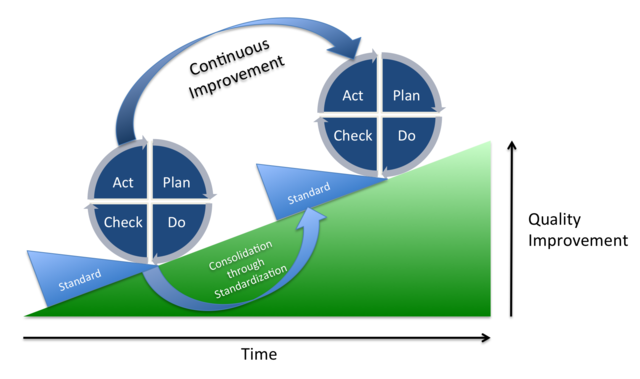
\includegraphics[width=1\textwidth]{PDCA.png}
	\caption{Continuous quality improvement with PDCA}
	\end{figure}
	
	\begin{enumerate}
		\item \textbf{PLAN}: vengono stabiliti gli obiettivi e i processi necessari per raggiungere i risultati attesi;
		\item \textbf{DO}: viene implementato il punto precedente, creando una parte del prodotto. In questo stadio vanno misurate le metriche;
		\item \textbf{CHECK}: vengono studiate ed elaborate le metriche rilevate al punto precedente, un confronto con i risultati attesi sarà il riscontro se quanto operato va nella direzione giusta. Vanno considerate metriche come la \emph{Schedule Variance} (vedi \ref{ScheduleVariance}) e la completezza dei risultati attesi soddisfatti, vanno elaborati grafici e tabelle per avere una visione chiara di quanto rilevato;
		\item \textbf{ACT}: vengono svolte le azioni correttive emerse dall'analisi del punto precedente e tutti i membri del gruppo vengono informati. Si potrà eseguire tramite riunioni o strumenti di messaggistica interna al gruppo. Terminato questo stadio si procederà con una nuova iterazione a partire dal punto 1.
	\end{enumerate}

	\subsection{Qualità dei processi}
	Definita in ISO/IEC 15504 come \glossario{SPICE}, specifica come la qualità è collegata alla maturazione dei processi, vengono individuati dei livelli di maturità al quale il fornitore può fare riferimento per determinare le proprie capacità organizzative. Vengono definiti:
	\begin{itemize}
		\item dei \textbf{Modelli di riferimento} su:
			\begin{itemize}
				\item \emph{dimensione del processo};
				\item \emph{livelli di capacità dei processi}:
					\begin{etaremune}
						\item ottimizzato
						\item predicibile
						\item stabilito
						\item gestito
						\item eseguito
						\item incompleto
					\end{etaremune}
					La capacità di un processo viene misurata tramite degli attributi che sono assimilabili alle metriche dei processi individuate in \ref{MetricheProcessi}, in particolare la \emph{Schedule Variance} permette di capire se un processo è incompleto o gestito; il gruppo giungerà a maturazione quando i processi diventeranno predicibili ossia quando la \emph{Schedule Variance} subirà al più lievi oscillazioni.
			\end{itemize}
		\item delle \textbf{Stime} che si concretizzano in una struttura per la misurazione composta da:
			\begin{itemize}
				\item i \emph{processi} di misurazione, indicati nel \PianoDiProgetto ;
				\item un \emph{modello} per la misurazione identificabile in questo documento;
				\item gli \emph{strumenti} utilizzati, specificati nelle \NormeDiProgetto .
			\end{itemize}
		\item le \textbf{Competenze e Qualifiche} di chi controlla; lo standard redige in modo rigoroso una serie di attività volte a formare chi opera l'attività di stesura del \emph{Piano di Qualifica} e \emph{Verifica}. Tali competenze sono assenti all'interno del gruppo e considerato che effettuare una formazione in linea con quanto specificato dallo standard sarebbe impossibile, tutti i membri si impegnano a studiare ed applicare al meglio quanto descritto in questo documento.
	\end{itemize}
	
	\subsection{Qualità del prodotto software}
	Specificata in ISO/IEC 9126 si suddivide in:
	\begin{itemize}
		\item \textbf{Quality model}: classifica la qualità del software in un set di caratteristiche che verranno approfondite nel corso del progetto:
			\begin{itemize}
				\item Functionality;
				\item Reliability;
				\item Usability;
				\item Efficiency;
				\item Maintainability;
				\item Portability.
			\end{itemize}
			Allo stato attuale, il gruppo non è in grado individuare un modello specifico per lo \glossario{stack} tecnologico da utilizzare.
		\item \textbf{External metrics}: sono le metriche rilevate tramite analisi dinamica, verranno specificate con il concretizzarsi della \emph{Specifica Tecnica};
		\item \textbf{Internal metrics}: sono le metriche rilevate in analisi statica specificate in \ref{MisureMetriche};
		\item \textbf{Quality in use metrics}: si tratta di metriche rilevabili allo stato di prodotto \emph{usabile} in condizioni reali, si rimanda la definizione di tale aspetto a quando verranno trattate le considerazioni sull'usabilità del prodotto in uno scenario di utilizzo reale, questo deve avvenire non oltre la \emph{Progettazione di Dettaglio e Codifica}.
	\end{itemize}



\section{PDCA}
\label{appendiceQualità}
In questo capitolo verrà descritto come è stato applicato il modello \glossario{PDCA} descritto nel \PianoDiQualifica.

\subsection{Revisione dei requisiti}

In questo periodo è stata svolta un attività di \emph{walkthrough} non avendo i dati necessari per effettuare attività di \emph{inspection}, come descritto nel \PianoDiQualifica. Gli errori frequenti rilevati sono visionabili nelle \NormeDiProgetto.

Non è stato possibile eseguire nessun ciclo \glossario{PDCA} in mancanza di misurazioni sui processi, non avendo quindi modo di pianificare processi per la qualità, ma è stato studiato e descritto nel \PianoDiQualifica{} e verrà attuato dalla prossima \glossario{milestone}.

\subsection{Revisione di progettazione}

\subparagraph{PLAN}

Al fine di valutare su quali processi pianificare dei miglioramenti sono state eseguite diverse misurazioni utilizzando le metriche per i processi descritte nel \PianoDiQualifica{}.

I risultati ottenuti sono riportati nella seguente tabella:

\begin{table}[H]
\centering
\begin{tabular}{ | c | c | c | }
\hline
\textbf{Metrica} & \textbf{Valore indice} & \textbf{Esito} \\
\hline
Produttività di documentazione & 199 & Superato \\
\hline
Impegno & 0,71 & Superato \\
\hline
Modifiche & 23 & Non superato \\
\hline
\end{tabular}
\caption{Risultati metriche per i processi, Revisione di progettazione}
\end{table}

Analizzando tali dati si è deciso di pianificare le seguenti attività per il miglioramento della qualità dei processi:

Un numero troppo elevato di modifiche incide pesantemente sulla produttività. È necessario decrementare tale valore al fine di aumentare la produttività e di conseguenza diminuire i costi. Questo primo ciclo \glossario{PDCA} si prefigge dunque l'obiettivo di portare entro un range di accettazione\footnote{Vedi \PianoDiQualifica} il numero di modifiche approvate.

Probabilmente un numero elevato di modifiche è causato dall'inesperienza del gruppo nel primo periodo, e ragionevolmente con l'aumentare delle conoscenze il numero di modifiche andrà calando di conseguenza. 

In ogni caso, si pianifica di:
\begin{itemize}
\item Frammentare maggiormente i task assegnati in sotto-task;
\item Specificare in modo esteso cosa prevede ogni singolo sotto-task, escludendo quindi dubbi che poi porteranno a successive richieste di modifica;
\item Creare la label ``Domanda'' nella sezione \glossario{issue} di \glossario{GitHub}, per permettere la richiesta di delucidazioni sullo svolgimento di \glossario{task} assegnati.
\end{itemize}
  
\subparagraph{CHECK}

Al fine di valutare se le azioni pianificate hanno portato ad un miglioramento dei processi sono state eseguite le necessarie misurazioni.

I risultati ottenuti sono riportati nella seguente tabella:
\begin{table}[H]
\centering
\begin{tabular}{ | c | c | c | }
\hline
\textbf{Metrica} & \textbf{Valore indice} & \textbf{Esito} \\
\hline
Produttività di documentazione & 103 & Superato \\
\hline
Impegno & 2,69 & Superato \\
\hline
Modifiche & 18 & Superato \\
\hline
\end{tabular}
\caption{Risultati metriche per i processi, Revisione di progettazione}
\end{table}

Gli obiettivi posti nello stadio di pianificazione sono stati soddisfatti, si passerà dunque allo stadio di standardizzazione delle soluzioni applicate.


\newpage
\subsection{Revisione di qualifica}
	\subparagraph{PLAN}
	La revisione di qualifica prevede la stesura della Definizione di Prodotto, la manualistica del prodotto e la relativa codifica. La codifica è una una parte corposa e ci aspettiamo una variazione visibile degli indici misurati. All'inizio della progettazione il gruppo si è accorto che l' autoformazione svolta non era sufficiente per poter progettare e successivamente codificare il prodotto richiesto. \`E stato così deciso di sviluppare, in un paio di giorni, un piccolo prototipo usa e getta che dovrebbe permettere di comprendere meglio lo stack tecnologico scelto. 
	
	
	\subparagraph{CHECK}
	Nell ambito del controllo dei cicli PDCA, viene introdotta in questa revisione un analisi delle issues di \glossario{GitHub} tramite un grafico di \glossario{burndown}. Viene rappresentato il carico di lavoro in relazione al tempo considerando sia il consuntivo sia il backlog, permettendo di confrontare l'andamento reale con quello atteso a fine fine milestone.
	
	\begin{figure}[h]
		\centering 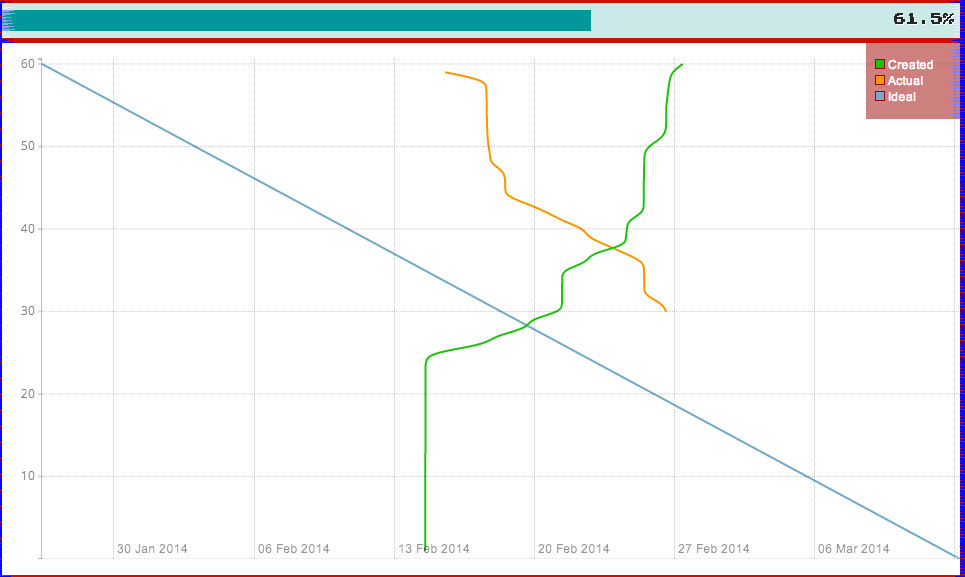
\includegraphics[width=0.8\textwidth]{burndownRQ.png}
		\caption{Burndown RQ}
	\end{figure}
	
	
	Per le metriche rilevate a fine della progettazione di dettaglio e codifica sono riportate nella seguente tabella:
\begin{table}[H]
\centering
\begin{tabular}{ | c | c | c | }
\hline
\textbf{Metrica} & \textbf{Valore indice} & \textbf{Esito} \\
\hline
Produttività di documentazione & 110 &  Superato \\
\hline
Produttività di codifica & 2.3 &  Superato \\
\hline
Impegno & 6.3 & Superato \\
\hline
Modifiche & 28 & Non superato \\
\hline
\end{tabular}
\caption{Risultati metriche Revisione di qualifica.}
\end{table}
	
	


% \subparagraph{PLAN}

% Al fine di valutare su quali processi pianificare dei processi di miglioramento sono state eseguite diverse misurazioni utilizzando le metriche per i processi descritti nel \PianoDiQualifica.

% I risultati ottenuti sono riportati nella seguente tabella:

% %TODO Completare tabella 

% \begin{tabular}{ | c | c | c | }
% \hline
% Documento & Valore indice & Esito \\
% \hline
% Produttività di documentazione & ?? & ?? \\
% \hline
% Impegno & ?? & ?? \\
% \hline
% Modifiche & ?? & ?? \\
% \hline
% \end{tabular}

% %\subsection{Revisione di accettazione}


\section{Use Case Points}

La metrica Use Case Points è stata applicata al fine di valutare l'attuabilità dello sviluppo di quali e quanti requisiti prima dell'accettazione.

Segue un breve studio di fattibilità basato sui risultati derivanti dall'applicazione degli Use Case Points.


\subsection{Fattori tecnici dell'implementazione}

I 13 fattori tecnici valutati sono:

\begin{enumerate}
	\item \textbf{Distributed System Required}: l'architettura della soluzione può essere centralizzata o single-tenant, o può essere distribuita (come una soluzione n-tier) o multi-tenant. Numeri più alti rappresentano un'architettura più complessa;
	\item \textbf{Response Time Is Important}: la rapidità di risposta per gli utenti è un fattore importante (e non banale). Ad esempio, se il carico del server dovrebbe essere molto bassa, questo può essere un fattore banale. Numeri alti rappresentano un'alta importanza del tempo di risposta;
	\item \textbf{End User Efficiency}: l'applicazione è sviluppata per migliorare l'efficienza d'uso, o semplicemente la capacità? Numeri alti rappresentano progetti che si basano più pesantemente sull'applicazione per migliorare l'efficienza d'uso;
	\item \textbf{Complex Internal Processing Required}: ci sono molti algoritmi complessi da implementare e testare? Algoritmi complessi hanno numeri alti. Delle semplici query al database dovrebbero avere numeri bassi;
	\item \textbf{Reusable Code Must Be a Focus}: il riuso massivo del codice è un obiettivo? Maggiore è il riuso del codice, minore è il valore relativo;
	\item \textbf{Installation Ease}: un'installazione agevole è un fattore chiave? Maggiore è il livello di competenza degli utenti, minore è il valore relativo;
	\item \textbf{Usability}: la facilità di utilizzo è un criterio primario per l'accettazione? Maggiore è l'importanza dell'usabilità, maggiore è il valore relativo;
	\item \textbf{Cross-Platform Support}: è richiesto il supporto multi-piattaforma? Più piattaforme devono essere supportate, più alto è il valore relativo;
	\item \textbf{Easy To Change}: il fornitore richiede di poter cambiare o personalizzare l'applicazione in futuro? Più richieste sono mosse in questa direzione, maggiore è il valore relativo;
	\item \textbf{Highly Concurrent}: bisogna preoccuparsi di questioni di concorrenza? Più attenzione bisogna prestare a risolvere conflitti su dati o sull'applicazione, maggiore è il valore relativo;
	\item \textbf{Custom Security}: è possibile utilizzare soluzioni già esistenti riguardanti la sicurezza o è necessario svilupparne di personali? Maggiori soluzioni personalizzare si devono implementare, più alto è il valore relativo;
	\item \textbf{Dependence on Third Party Code}: l'applicazione necessita l'uso di librerie o altro di terze parti? Più codice di terze parti (e più affidabile è), minore è li valore relativo;
	\item \textbf{User Training}: quanta formazione dell'utente è richiesta? L'applicazione è complessa o supporta attività complesse? Più tempo l'utente impiega nella formazione, maggiore è il valore relativo. 
\end{enumerate}

Per ogni fattore è necessario attribuire un valore da 0 a 5 che costituisce l'importanza relativa.

Il Technical Complexity Factor è calcolato sommando le importanze relative moltiplicate per il peso corrispondente, diviso per 100 e sommato a 0,6.

\begin{table}[H]
\begin{adjustwidth}{-4cm}{-4cm}
	\begin{center}
		\begin{tabular}{|c|c|c|c|c|}
			\hline
			\multicolumn{ 2}{|c|}{\raisebox{-1\height}{\textbf{Fattori tecnici}}} & \multicolumn{ 1}{c|}{\raisebox{-1\height}{\textbf{Peso}}} & \multicolumn{ 2}{c|}{\textbf{Importanza relativa}} \\ \cline{ 4- 5}
			\multicolumn{ 2}{|c|}{} & \multicolumn{ 1}{c|}{} & \textbf{Con tutti i requisiti} & \textbf{Solo requisiti acc.} \\ \hline
			1 & Distributed System Required & 2 & \textbf{4} & \textbf{0} \\ \hline
			2 & Response Time Is Important & 1 & \textbf{1} & \textbf{1} \\ \hline
			3 & End User Efficiency & 1 & \textbf{3} & \textbf{3} \\ \hline
			4 & Complex Internal Processing Required & 1 & \textbf{1} & \textbf{1} \\ \hline
			5 & Reusable Code Must Be A Focus & 1 & \textbf{2} & \textbf{2} \\ \hline
			6 & Installation Ease & 0.5 & \textbf{1} & \textbf{1} \\ \hline
			7 & Usability & 0.5 & \textbf{3} & \textbf{3} \\ \hline
			8 & Cross-Platform Support & 2 & \textbf{4} & \textbf{4} \\ \hline
			9 & Easy To Change & 1 & \textbf{1} & \textbf{1} \\ \hline
			10 & Highly Concurrent & 1 & \textbf{1} & \textbf{1} \\ \hline
			11 & Custom Security & 1 & \textbf{2} & \textbf{2} \\ \hline
			12 & Dependence On Third-Party Code & 1 & \textbf{2} & \textbf{2} \\ \hline
			13 & User Training & 1 & \textbf{3} & \textbf{2} \\ \hline
			\multicolumn{ 3}{|c|}{\textbf{Technical Complexity Factor}} & \textbf{0.94} & \textbf{0.85} \\ \hline
		\end{tabular}
	\end{center}
\caption{UCP - Fattori tecnici}
\end{adjustwidth}
\end{table}

I fattori che variano sono \emph{Distributed System Required} poiché non verrà implementato \glossario{MaaS} e \emph{User Training} in quanto la formazione degli utenti dovrà trattare di una minore mole di materiale.


\subsection{Fattori ambientali}

Gli 8 fattori ambientali valutati sono:

\begin{enumerate}
	\item \textbf{Familiarity With The Project}: quanta esperienza ha maturato il team nel dominio di sviluppo? Un alto livello di esperienza corrisponde ad un numero alto;
	\item \textbf{Application Experience}: quanta esperienza ha maturato il team con l'applicazione? Questo è rilevante solo quando si attuano cambiamenti a applicazioni già esistenti. Un valore alto corrisponde a molta esperienza;
	\item \textbf{Object Oriented Programming Experience}: quanta esperienza ha maturato il team verso l'Object Oriented? Un valore alto corrisponde a molta esperienza nell'Object Oriented;
	\item \textbf{Lead Analyst Capability}: quanto è esperto e abile la persona responsabile dei requisiti? Un valore alto rappresenta abilità e esperienza;
	\item \textbf{Motivation}: quanto è motivato il team? Un valore alto corrisponde a molta motivazione;
	\item \textbf{Stable Requirements}: cambiamenti nei requisiti comportano un incremento della mole di lavoro. Un valore alto corrisponde a molti cambiamenti;
	\item \textbf{Part Time Staff}: un valore alto riflette un team part time, consulenti esterni e sviluppatori che si occupano contemporaneamente di più progetti. Un cambiamento di contesto è causa di inefficienza;
	\item \textbf{Difficult Programming Language}: linguaggi di programmazione complessi corrispondono a numeri elevati. Questo valore è da attribuire in relazione alle capacità del team e non in senso assoluto.
\end{enumerate}

Per ogni fattore è necessario attribuire un valore da 0 a 5 che costituisce l'importanza relativa.

Ponendo $S$ la somma delle importanze relative moltiplicate per il peso corrispondente, l'Environmental Factor viene così calcolato:

\[
EF=1.4-(0.03 \cdot S)
\]

\begin{table}[H]
\begin{adjustwidth}{-4cm}{-4cm}
	\begin{center}
		\begin{tabular}{|c|c|c|c|c|}
			\hline
			\multicolumn{ 2}{|c|}{\raisebox{-1\height}{\textbf{Fattori ambientali}}} & \multicolumn{ 1}{c|}{\raisebox{-1\height}{\textbf{Peso}}} & \multicolumn{ 2}{c|}{\textbf{Importanza relativa}} \\ \cline{ 4- 5}
			\multicolumn{ 2}{|c|}{\textbf{}} & \multicolumn{ 1}{c|}{} & \textbf{Con tutti i requisiti} & \textbf{Solo requisiti acc.} \\ \hline
			1 & Familiarity With The Project & 1.5 & \textbf{0} & \textbf{0} \\ \hline
			2 & Application Experience & 0.5 & \textbf{0} & \textbf{0} \\ \hline
			3 & OO Programming Experience & 1 & \textbf{1} & \textbf{1} \\ \hline
			4 & Lead Analyst Capability & 0.5 & \textbf{1} & \textbf{1} \\ \hline
			5 & Motivation & 1 & \textbf{5} & \textbf{5} \\ \hline
			6 & Stable Requirements & 2 & \textbf{2} & \textbf{3} \\ \hline
			7 & Part Time Staff & -1 & \textbf{3} & \textbf{3} \\ \hline
			8 & Difficult Programming Language & -1 & \textbf{5} & \textbf{5} \\ \hline
			\multicolumn{ 3}{|c|}{\textbf{Environmental Factor}} & \textbf{1.325} & \textbf{1.265} \\ \hline
		\end{tabular}
	\end{center}
\caption{UCP - Fattori ambientali}
\end{adjustwidth}
\end{table}

L'unico fattore che varia è \emph{Stable Requirements} poiché un maggior numero di requisiti porta ad una maggiore probabilità di cambiamento degli stessi.


\subsection{Quantità e complessità degli use case}

Ad ogni use case valutato viene attribuito un numero di \emph{use case points} in base al suo grado di complessità, calcolato sul numero di transazioni, inteso come scambio, una risposta del sistema ad un'azione dell'utente:

\begin{itemize}
	\item \textbf{Simple}: fino a 3 transazioni;
	\item \textbf{Average}: da 4 a 7 transazioni;
	\item \textbf{Complex}: più di 7 transazioni.
\end{itemize}

Il calcolo degli Unadjusted Use Case Points è uguale alla somma delle importanze relative moltiplicate per il peso corrispondente.

\begin{table}[H]
\begin{adjustwidth}{-4cm}{-4cm}
	\begin{center}
		\begin{tabular}{|c|c|c|c|c|}
			\hline
			\multicolumn{ 2}{|c|}{\raisebox{-1\height}{\textbf{Use Case Points grezzi}}} & \multicolumn{ 1}{c|}{\raisebox{-1\height}{\textbf{Peso}}} & \multicolumn{ 2}{c|}{\textbf{Numero di use case}} \\ \cline{ 4- 5}
			\multicolumn{ 2}{|c|}{\textbf{}} & \multicolumn{ 1}{c|}{} & \textbf{Con tutti i requisiti} & \textbf{Solo requisiti acc.} \\ \hline
			1 & Simple & 5 & \textbf{21} & \textbf{15} \\ \hline
			2 & Average & 10 & \textbf{1} & \textbf{1} \\ \hline
			3 & Complex & 15 & \textbf{0} & \textbf{0} \\ \hline
			\multicolumn{ 3}{|c|}{\textbf{Unadjusted Use Case Points}} & \textbf{115} & \textbf{85} \\ \hline
		\end{tabular}
	\end{center}
\caption{UCP - Quantità e complessità degli use case}
\end{adjustwidth}
\end{table}

Il tracciamento dei requisiti riportato in \AnalisiDeiRequisiti{} permette di non considerare i casi d'uso che sono legati a requisiti non accettati.


\subsection{Quantità e complessità degli attori}

Ad ogni attore valutato viene attribuito un peso in base al suo grado di complessità:

\begin{itemize}
	\item \textbf{Simple}: sono altri sistemi che comunicano con il proprio software attraverso delle \glossario{API} predefinite. L'elemento chiave è che si sta esponendo un'interazione con il proprio software attraverso un meccanismo specifico e ben definito;
	\item \textbf{Average}: possono essere sia uomini che interagiscono con un protocollo ben definito, sia sistemi che utilizzano \glossario{API} più complesse o flessibili;
	\item \textbf{Complex}: utenti che interagiscono con il sistema in modo imprevedibile anche attraverso interfacce grafiche.
\end{itemize}

Il calcolo dell'Actor Complexity Factor è uguale alla somma delle importanze relative moltiplicate per il peso corrispondente.

\begin{table}[H]
\begin{adjustwidth}{-4cm}{-4cm}
	\begin{center}
		\begin{tabular}{|c|c|c|c|c|}
			\hline
			\multicolumn{ 2}{|c|}{\raisebox{-1\height}{\textbf{Attori}}} & \multicolumn{ 1}{c|}{\raisebox{-1\height}{\textbf{Peso}}} & \multicolumn{ 2}{c|}{\textbf{Number of Actors}} \\ \cline{ 4- 5}
			\multicolumn{ 2}{|c|}{\textbf{}} & \multicolumn{ 1}{c|}{} & \textbf{Con tutti i requisiti} & \textbf{Solo requisiti acc.} \\ \hline
			1 & Simple & 1 & \textbf{0} & \textbf{0} \\ \hline
			2 & Average & 2 & \textbf{1} & \textbf{1} \\ \hline
			3 & Complex & 3 & \textbf{6} & \textbf{4} \\ \hline
			\multicolumn{ 3}{|c|}{\textbf{Actor Complexity Factor}} & \textbf{20} & \textbf{14} \\ \hline
		\end{tabular}
	\end{center}
\caption{UCP - Quantità e complessità degli attori}
\end{adjustwidth}
\end{table}

Gli attori implicati nell'interazione con il sistema \glossario{MaaS} non vengono calcolati. Il fattore di complessità risulta diminuire sensibilmente considerando solo i requisiti accettati poiché gli utenti \glossario{MaaS} sono ritenuti \emph{complessi}.


\subsection{Risultati e conclusioni}

Ponendo

\begin{itemize}
	\item Technical Complexity Factor = $TCF$;
	\item Environmental Factor = $EF$;
	\item Unadjusted Use Case Points = $UUCP$;
	\item Actor Complexity Factor = $ACF$;
	\item Use Case Points = $UCP$;
	\item Ore di impegno per Use Case Point = $HUCP$;
\end{itemize}

il calcolo delle ore di impegno sarà

\[
Ore = [ (UUCP+ACF) \cdot TCF \cdot EF ] \cdot HUCP
\]

\begin{table}[H]
\begin{adjustwidth}{-4cm}{-4cm}
	\begin{center}
		\begin{tabular}{|r|r|r|r|}
			\hline
			\multicolumn{ 4}{|c|}{\textbf{Fattori di complessità}} \\ \hline
			TCF & Technical Complexity Factor & 0.94 & 0.85 \\ \hline
			EF & Environmental Factor & 1.325 & 1.265 \\ \hline
			UUCP & Unadjusted Use Case Points & 115 & 85 \\ \hline
			ACF & Actor Complexity Factor & 20 & 14 \\ \hline
			\multicolumn{ 4}{|c|}{\textbf{Calcolo Use Case Points}} \\ \hline
			UCP & Use Case Points & 168.1 & 106.4 \\ \hline
			\multicolumn{ 4}{|c|}{\textbf{Calcolo ore di sviluppo}} \\ \hline
			Rapporto & Ore di impegno per Use Case Point & 7 & 7 \\ \hline
			\multicolumn{ 4}{|c|}{} \\ \hline
			\multicolumn{ 2}{|r|}{\textbf{Ore di impegno}} & \textbf{ 1,177 } & \textbf{ 745 } \\ \hline
		\end{tabular}
	\end{center}
\caption{UCP - Ore di impegno stimate}
\label{tab:UCP-ore-di-impegno-stimate}
\end{adjustwidth}
\end{table}

I risultati riportati in tabella \ref{tab:UCP-ore-di-impegno-stimate} mettono in evidenza come le ore necessarie per lo sviluppo di tutti i requisiti richieda uno sforzo quantificato in ore non sostenibile per il gruppo, e che eccede eccessivamente il limite superiore delle 105 ore produttive per ciascun componente del gruppo. Considerando solo i requisiti accettati (vedi \AnalisiDeiRequisiti), si nota come le ore di impegno scendano ad un livello molto vicino alle attese. Dal momento che la quantificazione risultante dalla tecnica utilizzata è una stima, è plausibile ritenere accettabile tale livello e procedere verso la direzione scelta con l'accettazione dei requisiti.

%\pagebreak


% TS / req
	
	\begin{table}[h]
		\begin{tabularx}{\textwidth}{ | c | P{3cm} | c | X | }
 			\hline \textbf{Test} & \textbf{Descrizione} & \textbf{Stato} & \textbf{Requisito} \\ % INTESTAZIONE TABELLA
 				\hline col1 & col2 & col3 & col4 \\ % <------ CONTENUTO
 			\hline % obbligatorio alla fine !
		\end{tabularx}
		\caption{Associazione test di sistema con relativo requisito.}
	\end{table}
	
	
	
% TI / componente

	\begin{table}[h]
		\begin{tabularx}{\textwidth}{ | c | P{3cm} | c | X | }
 			\hline \textbf{Test} & \textbf{Descrizione} & \textbf{Componente} & \textbf{Stato} \\ % INTESTAZIONE TABELLA
 				\hline col1 & col2 & col3 & col4 \\ % <------ CONTENUTO
 			\hline % obbligatorio alla fine !
		\end{tabularx}
		\caption{Associazione test di integrazione con relativo componente.}
	\end{table}

% componente / TI
	\begin{table}[h]
		\begin{tabularx}{\textwidth}{ | X | X | }
 			\hline \textbf{Componente} & \textbf{Test}  \\ % INTESTAZIONE TABELLA
 				\hline col1 & col2 \\ % <------ CONTENUTO
 			\hline % obbligatorio alla fine !
		\end{tabularx}
		\caption{Tracciamento componenti test di integrazione.}
	\end{table}

% TV



\textbf{NOME TEST PRIMO LIVELLO} % PRIMO LVL = TVx
\begin{center}
      \bgroup
      \def\arraystretch{1.3}
	\begin{longtable}{ p{2.3cm} p{10cm} }
		\textbf{Scopo:} & TESTO SCOPO \\ % TESTO SCOPO TV primo livello
		\textbf{Dipendenze:} & TESTO DIPENDENZE \\ % TESTO DIP. TV primo livevllo
		\textbf{All'utente è richiesto di:} &
			\begin{itemize} % ELENCO PUNTATO DEI TEST FIGLI IN MODO RICORSIVO cioè per ogni livello va un sotto-elenco puntato.
				\item TESTO DESCRIZIONE TV DI LIVELLO 2  (TV x.x) % TESTO DESCR + CODICE TV secondo livello!
			\end{itemize}
	\end{longtable}
      \egroup
\end{center}  



 % è qui solo per testare rapidamente i template delle tabelle dei test

\end{document}


